% Created by tikzDevice version 0.12.6 on 2025-02-16 17:47:45
% !TEX encoding = UTF-8 Unicode
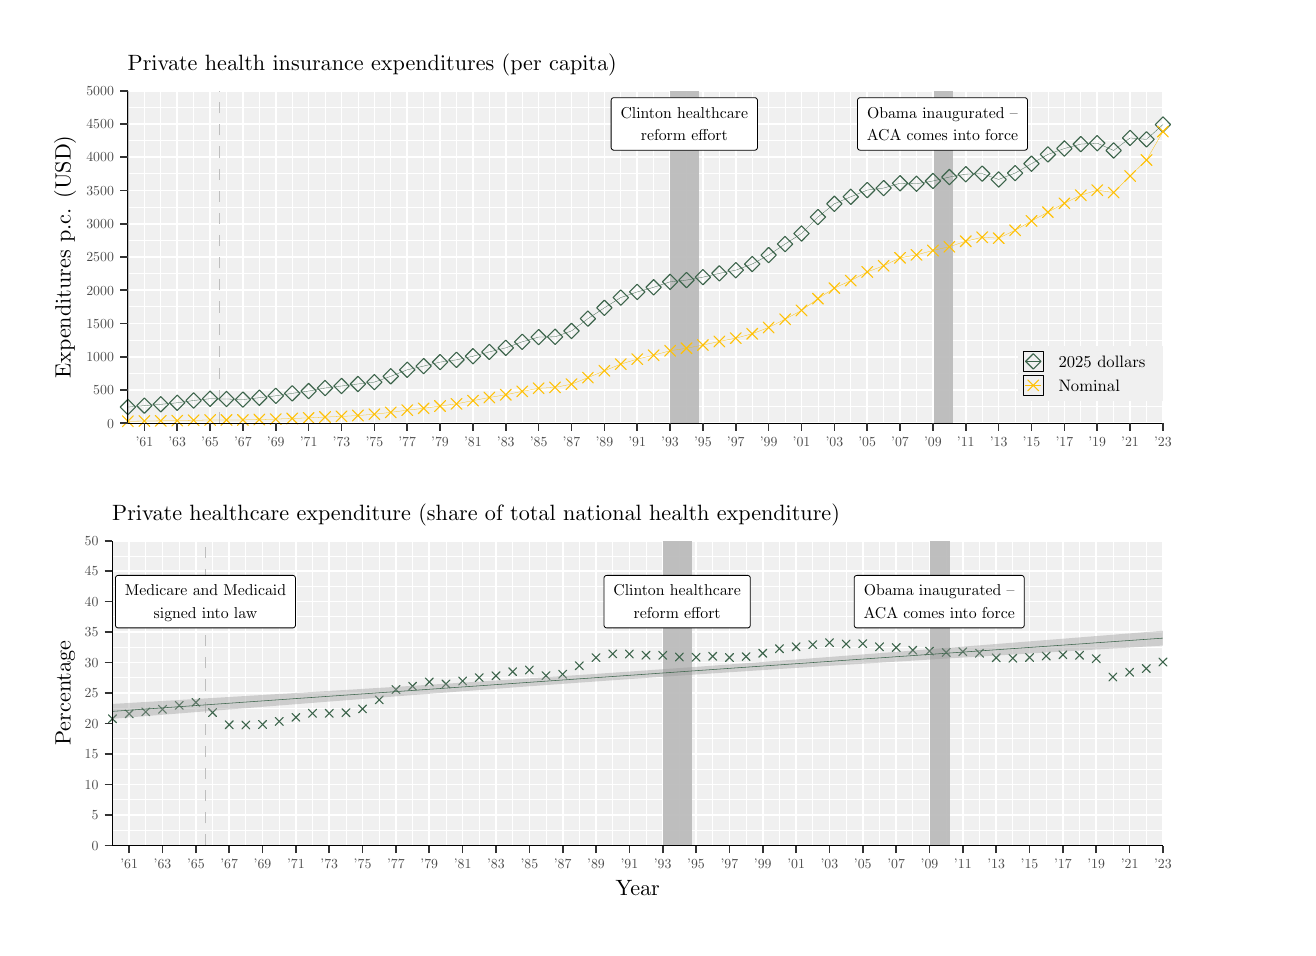
\begin{tikzpicture}[x=1pt,y=1pt]
\definecolor{fillColor}{RGB}{255,255,255}
\path[use as bounding box,fill=fillColor,fill opacity=0.00] (0,0) rectangle (455.30,325.21);
\begin{scope}
\path[clip] (  0.00,162.61) rectangle (455.30,325.21);
\definecolor{drawColor}{RGB}{255,255,255}
\definecolor{fillColor}{RGB}{255,255,255}

\path[draw=drawColor,line width= 0.6pt,line join=round,line cap=round,fill=fillColor] (  0.00,162.61) rectangle (455.30,325.21);
\end{scope}
\begin{scope}
\path[clip] (  0.00,  0.00) rectangle (455.30,325.21);
\definecolor{fillColor}{gray}{0.94}

\path[fill=fillColor] ( 36.14,182.27) rectangle (410.30,302.44);
\definecolor{drawColor}{RGB}{255,255,255}

\path[draw=drawColor,line width= 0.3pt,line join=round] ( 36.14,188.27) --
	(410.30,188.27);

\path[draw=drawColor,line width= 0.3pt,line join=round] ( 36.14,200.29) --
	(410.30,200.29);

\path[draw=drawColor,line width= 0.3pt,line join=round] ( 36.14,212.31) --
	(410.30,212.31);

\path[draw=drawColor,line width= 0.3pt,line join=round] ( 36.14,224.33) --
	(410.30,224.33);

\path[draw=drawColor,line width= 0.3pt,line join=round] ( 36.14,236.34) --
	(410.30,236.34);

\path[draw=drawColor,line width= 0.3pt,line join=round] ( 36.14,248.36) --
	(410.30,248.36);

\path[draw=drawColor,line width= 0.3pt,line join=round] ( 36.14,260.38) --
	(410.30,260.38);

\path[draw=drawColor,line width= 0.3pt,line join=round] ( 36.14,272.40) --
	(410.30,272.40);

\path[draw=drawColor,line width= 0.3pt,line join=round] ( 36.14,284.41) --
	(410.30,284.41);

\path[draw=drawColor,line width= 0.3pt,line join=round] ( 36.14,296.43) --
	(410.30,296.43);

\path[draw=drawColor,line width= 0.3pt,line join=round] ( 36.23,182.27) --
	( 36.23,302.44);

\path[draw=drawColor,line width= 0.3pt,line join=round] ( 48.10,182.27) --
	( 48.10,302.44);

\path[draw=drawColor,line width= 0.3pt,line join=round] ( 59.97,182.27) --
	( 59.97,302.44);

\path[draw=drawColor,line width= 0.3pt,line join=round] ( 71.85,182.27) --
	( 71.85,302.44);

\path[draw=drawColor,line width= 0.3pt,line join=round] ( 83.72,182.27) --
	( 83.72,302.44);

\path[draw=drawColor,line width= 0.3pt,line join=round] ( 95.59,182.27) --
	( 95.59,302.44);

\path[draw=drawColor,line width= 0.3pt,line join=round] (107.46,182.27) --
	(107.46,302.44);

\path[draw=drawColor,line width= 0.3pt,line join=round] (119.34,182.27) --
	(119.34,302.44);

\path[draw=drawColor,line width= 0.3pt,line join=round] (131.21,182.27) --
	(131.21,302.44);

\path[draw=drawColor,line width= 0.3pt,line join=round] (143.08,182.27) --
	(143.08,302.44);

\path[draw=drawColor,line width= 0.3pt,line join=round] (154.96,182.27) --
	(154.96,302.44);

\path[draw=drawColor,line width= 0.3pt,line join=round] (166.83,182.27) --
	(166.83,302.44);

\path[draw=drawColor,line width= 0.3pt,line join=round] (178.70,182.27) --
	(178.70,302.44);

\path[draw=drawColor,line width= 0.3pt,line join=round] (190.58,182.27) --
	(190.58,302.44);

\path[draw=drawColor,line width= 0.3pt,line join=round] (202.45,182.27) --
	(202.45,302.44);

\path[draw=drawColor,line width= 0.3pt,line join=round] (214.32,182.27) --
	(214.32,302.44);

\path[draw=drawColor,line width= 0.3pt,line join=round] (226.19,182.27) --
	(226.19,302.44);

\path[draw=drawColor,line width= 0.3pt,line join=round] (238.07,182.27) --
	(238.07,302.44);

\path[draw=drawColor,line width= 0.3pt,line join=round] (249.94,182.27) --
	(249.94,302.44);

\path[draw=drawColor,line width= 0.3pt,line join=round] (261.81,182.27) --
	(261.81,302.44);

\path[draw=drawColor,line width= 0.3pt,line join=round] (273.69,182.27) --
	(273.69,302.44);

\path[draw=drawColor,line width= 0.3pt,line join=round] (285.56,182.27) --
	(285.56,302.44);

\path[draw=drawColor,line width= 0.3pt,line join=round] (297.43,182.27) --
	(297.43,302.44);

\path[draw=drawColor,line width= 0.3pt,line join=round] (309.30,182.27) --
	(309.30,302.44);

\path[draw=drawColor,line width= 0.3pt,line join=round] (321.18,182.27) --
	(321.18,302.44);

\path[draw=drawColor,line width= 0.3pt,line join=round] (333.05,182.27) --
	(333.05,302.44);

\path[draw=drawColor,line width= 0.3pt,line join=round] (344.92,182.27) --
	(344.92,302.44);

\path[draw=drawColor,line width= 0.3pt,line join=round] (356.80,182.27) --
	(356.80,302.44);

\path[draw=drawColor,line width= 0.3pt,line join=round] (368.67,182.27) --
	(368.67,302.44);

\path[draw=drawColor,line width= 0.3pt,line join=round] (380.54,182.27) --
	(380.54,302.44);

\path[draw=drawColor,line width= 0.3pt,line join=round] (392.41,182.27) --
	(392.41,302.44);

\path[draw=drawColor,line width= 0.3pt,line join=round] (404.29,182.27) --
	(404.29,302.44);

\path[draw=drawColor,line width= 0.6pt,line join=round] ( 36.14,182.27) --
	(410.30,182.27);

\path[draw=drawColor,line width= 0.6pt,line join=round] ( 36.14,194.28) --
	(410.30,194.28);

\path[draw=drawColor,line width= 0.6pt,line join=round] ( 36.14,206.30) --
	(410.30,206.30);

\path[draw=drawColor,line width= 0.6pt,line join=round] ( 36.14,218.32) --
	(410.30,218.32);

\path[draw=drawColor,line width= 0.6pt,line join=round] ( 36.14,230.33) --
	(410.30,230.33);

\path[draw=drawColor,line width= 0.6pt,line join=round] ( 36.14,242.35) --
	(410.30,242.35);

\path[draw=drawColor,line width= 0.6pt,line join=round] ( 36.14,254.37) --
	(410.30,254.37);

\path[draw=drawColor,line width= 0.6pt,line join=round] ( 36.14,266.39) --
	(410.30,266.39);

\path[draw=drawColor,line width= 0.6pt,line join=round] ( 36.14,278.40) --
	(410.30,278.40);

\path[draw=drawColor,line width= 0.6pt,line join=round] ( 36.14,290.42) --
	(410.30,290.42);

\path[draw=drawColor,line width= 0.6pt,line join=round] ( 36.14,302.44) --
	(410.30,302.44);

\path[draw=drawColor,line width= 0.6pt,line join=round] ( 42.17,182.27) --
	( 42.17,302.44);

\path[draw=drawColor,line width= 0.6pt,line join=round] ( 54.03,182.27) --
	( 54.03,302.44);

\path[draw=drawColor,line width= 0.6pt,line join=round] ( 65.91,182.27) --
	( 65.91,302.44);

\path[draw=drawColor,line width= 0.6pt,line join=round] ( 77.78,182.27) --
	( 77.78,302.44);

\path[draw=drawColor,line width= 0.6pt,line join=round] ( 89.66,182.27) --
	( 89.66,302.44);

\path[draw=drawColor,line width= 0.6pt,line join=round] (101.52,182.27) --
	(101.52,302.44);

\path[draw=drawColor,line width= 0.6pt,line join=round] (113.41,182.27) --
	(113.41,302.44);

\path[draw=drawColor,line width= 0.6pt,line join=round] (125.27,182.27) --
	(125.27,302.44);

\path[draw=drawColor,line width= 0.6pt,line join=round] (137.15,182.27) --
	(137.15,302.44);

\path[draw=drawColor,line width= 0.6pt,line join=round] (149.02,182.27) --
	(149.02,302.44);

\path[draw=drawColor,line width= 0.6pt,line join=round] (160.90,182.27) --
	(160.90,302.44);

\path[draw=drawColor,line width= 0.6pt,line join=round] (172.76,182.27) --
	(172.76,302.44);

\path[draw=drawColor,line width= 0.6pt,line join=round] (184.64,182.27) --
	(184.64,302.44);

\path[draw=drawColor,line width= 0.6pt,line join=round] (196.51,182.27) --
	(196.51,302.44);

\path[draw=drawColor,line width= 0.6pt,line join=round] (208.39,182.27) --
	(208.39,302.44);

\path[draw=drawColor,line width= 0.6pt,line join=round] (220.25,182.27) --
	(220.25,302.44);

\path[draw=drawColor,line width= 0.6pt,line join=round] (232.13,182.27) --
	(232.13,302.44);

\path[draw=drawColor,line width= 0.6pt,line join=round] (244.00,182.27) --
	(244.00,302.44);

\path[draw=drawColor,line width= 0.6pt,line join=round] (255.88,182.27) --
	(255.88,302.44);

\path[draw=drawColor,line width= 0.6pt,line join=round] (267.74,182.27) --
	(267.74,302.44);

\path[draw=drawColor,line width= 0.6pt,line join=round] (279.63,182.27) --
	(279.63,302.44);

\path[draw=drawColor,line width= 0.6pt,line join=round] (291.49,182.27) --
	(291.49,302.44);

\path[draw=drawColor,line width= 0.6pt,line join=round] (303.37,182.27) --
	(303.37,302.44);

\path[draw=drawColor,line width= 0.6pt,line join=round] (315.24,182.27) --
	(315.24,302.44);

\path[draw=drawColor,line width= 0.6pt,line join=round] (327.12,182.27) --
	(327.12,302.44);

\path[draw=drawColor,line width= 0.6pt,line join=round] (338.98,182.27) --
	(338.98,302.44);

\path[draw=drawColor,line width= 0.6pt,line join=round] (350.86,182.27) --
	(350.86,302.44);

\path[draw=drawColor,line width= 0.6pt,line join=round] (362.73,182.27) --
	(362.73,302.44);

\path[draw=drawColor,line width= 0.6pt,line join=round] (374.61,182.27) --
	(374.61,302.44);

\path[draw=drawColor,line width= 0.6pt,line join=round] (386.47,182.27) --
	(386.47,302.44);

\path[draw=drawColor,line width= 0.6pt,line join=round] (398.35,182.27) --
	(398.35,302.44);

\path[draw=drawColor,line width= 0.6pt,line join=round] (410.22,182.27) --
	(410.22,302.44);
\definecolor{drawColor}{RGB}{190,190,190}

\path[draw=drawColor,line width= 0.6pt,line join=round] ( 36.22,182.27) -- ( 36.22,302.44);
\definecolor{fillColor}{RGB}{190,190,190}

\path[fill=fillColor,fill opacity=0.01] (232.13,182.27) rectangle (242.42,302.44);

\path[fill=fillColor,fill opacity=0.01] (232.13,182.27) rectangle (242.42,302.44);

\path[fill=fillColor,fill opacity=0.01] (232.13,182.27) rectangle (242.42,302.44);

\path[fill=fillColor,fill opacity=0.01] (232.13,182.27) rectangle (242.42,302.44);

\path[fill=fillColor,fill opacity=0.01] (232.13,182.27) rectangle (242.42,302.44);

\path[fill=fillColor,fill opacity=0.01] (232.13,182.27) rectangle (242.42,302.44);

\path[fill=fillColor,fill opacity=0.01] (232.13,182.27) rectangle (242.42,302.44);

\path[fill=fillColor,fill opacity=0.01] (232.13,182.27) rectangle (242.42,302.44);

\path[fill=fillColor,fill opacity=0.01] (232.13,182.27) rectangle (242.42,302.44);

\path[fill=fillColor,fill opacity=0.01] (232.13,182.27) rectangle (242.42,302.44);

\path[fill=fillColor,fill opacity=0.01] (232.13,182.27) rectangle (242.42,302.44);

\path[fill=fillColor,fill opacity=0.01] (232.13,182.27) rectangle (242.42,302.44);

\path[fill=fillColor,fill opacity=0.01] (232.13,182.27) rectangle (242.42,302.44);

\path[fill=fillColor,fill opacity=0.01] (232.13,182.27) rectangle (242.42,302.44);

\path[fill=fillColor,fill opacity=0.01] (232.13,182.27) rectangle (242.42,302.44);

\path[fill=fillColor,fill opacity=0.01] (232.13,182.27) rectangle (242.42,302.44);

\path[fill=fillColor,fill opacity=0.01] (232.13,182.27) rectangle (242.42,302.44);

\path[fill=fillColor,fill opacity=0.01] (232.13,182.27) rectangle (242.42,302.44);

\path[fill=fillColor,fill opacity=0.01] (232.13,182.27) rectangle (242.42,302.44);

\path[fill=fillColor,fill opacity=0.01] (232.13,182.27) rectangle (242.42,302.44);

\path[fill=fillColor,fill opacity=0.01] (232.13,182.27) rectangle (242.42,302.44);

\path[fill=fillColor,fill opacity=0.01] (232.13,182.27) rectangle (242.42,302.44);

\path[fill=fillColor,fill opacity=0.01] (232.13,182.27) rectangle (242.42,302.44);

\path[fill=fillColor,fill opacity=0.01] (232.13,182.27) rectangle (242.42,302.44);

\path[fill=fillColor,fill opacity=0.01] (232.13,182.27) rectangle (242.42,302.44);

\path[fill=fillColor,fill opacity=0.01] (232.13,182.27) rectangle (242.42,302.44);

\path[fill=fillColor,fill opacity=0.01] (232.13,182.27) rectangle (242.42,302.44);

\path[fill=fillColor,fill opacity=0.01] (232.13,182.27) rectangle (242.42,302.44);

\path[fill=fillColor,fill opacity=0.01] (232.13,182.27) rectangle (242.42,302.44);

\path[fill=fillColor,fill opacity=0.01] (232.13,182.27) rectangle (242.42,302.44);

\path[fill=fillColor,fill opacity=0.01] (232.13,182.27) rectangle (242.42,302.44);

\path[fill=fillColor,fill opacity=0.01] (232.13,182.27) rectangle (242.42,302.44);

\path[fill=fillColor,fill opacity=0.01] (232.13,182.27) rectangle (242.42,302.44);

\path[fill=fillColor,fill opacity=0.01] (232.13,182.27) rectangle (242.42,302.44);

\path[fill=fillColor,fill opacity=0.01] (232.13,182.27) rectangle (242.42,302.44);

\path[fill=fillColor,fill opacity=0.01] (232.13,182.27) rectangle (242.42,302.44);

\path[fill=fillColor,fill opacity=0.01] (232.13,182.27) rectangle (242.42,302.44);

\path[fill=fillColor,fill opacity=0.01] (232.13,182.27) rectangle (242.42,302.44);

\path[fill=fillColor,fill opacity=0.01] (232.13,182.27) rectangle (242.42,302.44);

\path[fill=fillColor,fill opacity=0.01] (232.13,182.27) rectangle (242.42,302.44);

\path[fill=fillColor,fill opacity=0.01] (232.13,182.27) rectangle (242.42,302.44);

\path[fill=fillColor,fill opacity=0.01] (232.13,182.27) rectangle (242.42,302.44);

\path[fill=fillColor,fill opacity=0.01] (232.13,182.27) rectangle (242.42,302.44);

\path[fill=fillColor,fill opacity=0.01] (232.13,182.27) rectangle (242.42,302.44);

\path[fill=fillColor,fill opacity=0.01] (232.13,182.27) rectangle (242.42,302.44);

\path[fill=fillColor,fill opacity=0.01] (232.13,182.27) rectangle (242.42,302.44);

\path[fill=fillColor,fill opacity=0.01] (232.13,182.27) rectangle (242.42,302.44);

\path[fill=fillColor,fill opacity=0.01] (232.13,182.27) rectangle (242.42,302.44);

\path[fill=fillColor,fill opacity=0.01] (232.13,182.27) rectangle (242.42,302.44);

\path[fill=fillColor,fill opacity=0.01] (232.13,182.27) rectangle (242.42,302.44);

\path[fill=fillColor,fill opacity=0.01] (232.13,182.27) rectangle (242.42,302.44);

\path[fill=fillColor,fill opacity=0.01] (232.13,182.27) rectangle (242.42,302.44);

\path[fill=fillColor,fill opacity=0.01] (232.13,182.27) rectangle (242.42,302.44);

\path[fill=fillColor,fill opacity=0.01] (232.13,182.27) rectangle (242.42,302.44);

\path[fill=fillColor,fill opacity=0.01] (232.13,182.27) rectangle (242.42,302.44);

\path[fill=fillColor,fill opacity=0.01] (232.13,182.27) rectangle (242.42,302.44);

\path[fill=fillColor,fill opacity=0.01] (232.13,182.27) rectangle (242.42,302.44);

\path[fill=fillColor,fill opacity=0.01] (232.13,182.27) rectangle (242.42,302.44);

\path[fill=fillColor,fill opacity=0.01] (232.13,182.27) rectangle (242.42,302.44);

\path[fill=fillColor,fill opacity=0.01] (232.13,182.27) rectangle (242.42,302.44);

\path[fill=fillColor,fill opacity=0.01] (232.13,182.27) rectangle (242.42,302.44);

\path[fill=fillColor,fill opacity=0.01] (232.13,182.27) rectangle (242.42,302.44);

\path[fill=fillColor,fill opacity=0.01] (232.13,182.27) rectangle (242.42,302.44);

\path[fill=fillColor,fill opacity=0.01] (232.13,182.27) rectangle (242.42,302.44);

\path[fill=fillColor,fill opacity=0.01] (327.43,182.27) rectangle (334.37,302.44);

\path[fill=fillColor,fill opacity=0.01] (327.43,182.27) rectangle (334.37,302.44);

\path[fill=fillColor,fill opacity=0.01] (327.43,182.27) rectangle (334.37,302.44);

\path[fill=fillColor,fill opacity=0.01] (327.43,182.27) rectangle (334.37,302.44);

\path[fill=fillColor,fill opacity=0.01] (327.43,182.27) rectangle (334.37,302.44);

\path[fill=fillColor,fill opacity=0.01] (327.43,182.27) rectangle (334.37,302.44);

\path[fill=fillColor,fill opacity=0.01] (327.43,182.27) rectangle (334.37,302.44);

\path[fill=fillColor,fill opacity=0.01] (327.43,182.27) rectangle (334.37,302.44);

\path[fill=fillColor,fill opacity=0.01] (327.43,182.27) rectangle (334.37,302.44);

\path[fill=fillColor,fill opacity=0.01] (327.43,182.27) rectangle (334.37,302.44);

\path[fill=fillColor,fill opacity=0.01] (327.43,182.27) rectangle (334.37,302.44);

\path[fill=fillColor,fill opacity=0.01] (327.43,182.27) rectangle (334.37,302.44);

\path[fill=fillColor,fill opacity=0.01] (327.43,182.27) rectangle (334.37,302.44);

\path[fill=fillColor,fill opacity=0.01] (327.43,182.27) rectangle (334.37,302.44);

\path[fill=fillColor,fill opacity=0.01] (327.43,182.27) rectangle (334.37,302.44);

\path[fill=fillColor,fill opacity=0.01] (327.43,182.27) rectangle (334.37,302.44);

\path[fill=fillColor,fill opacity=0.01] (327.43,182.27) rectangle (334.37,302.44);

\path[fill=fillColor,fill opacity=0.01] (327.43,182.27) rectangle (334.37,302.44);

\path[fill=fillColor,fill opacity=0.01] (327.43,182.27) rectangle (334.37,302.44);

\path[fill=fillColor,fill opacity=0.01] (327.43,182.27) rectangle (334.37,302.44);

\path[fill=fillColor,fill opacity=0.01] (327.43,182.27) rectangle (334.37,302.44);

\path[fill=fillColor,fill opacity=0.01] (327.43,182.27) rectangle (334.37,302.44);

\path[fill=fillColor,fill opacity=0.01] (327.43,182.27) rectangle (334.37,302.44);

\path[fill=fillColor,fill opacity=0.01] (327.43,182.27) rectangle (334.37,302.44);

\path[fill=fillColor,fill opacity=0.01] (327.43,182.27) rectangle (334.37,302.44);

\path[fill=fillColor,fill opacity=0.01] (327.43,182.27) rectangle (334.37,302.44);

\path[fill=fillColor,fill opacity=0.01] (327.43,182.27) rectangle (334.37,302.44);

\path[fill=fillColor,fill opacity=0.01] (327.43,182.27) rectangle (334.37,302.44);

\path[fill=fillColor,fill opacity=0.01] (327.43,182.27) rectangle (334.37,302.44);

\path[fill=fillColor,fill opacity=0.01] (327.43,182.27) rectangle (334.37,302.44);

\path[fill=fillColor,fill opacity=0.01] (327.43,182.27) rectangle (334.37,302.44);

\path[fill=fillColor,fill opacity=0.01] (327.43,182.27) rectangle (334.37,302.44);

\path[fill=fillColor,fill opacity=0.01] (327.43,182.27) rectangle (334.37,302.44);

\path[fill=fillColor,fill opacity=0.01] (327.43,182.27) rectangle (334.37,302.44);

\path[fill=fillColor,fill opacity=0.01] (327.43,182.27) rectangle (334.37,302.44);

\path[fill=fillColor,fill opacity=0.01] (327.43,182.27) rectangle (334.37,302.44);

\path[fill=fillColor,fill opacity=0.01] (327.43,182.27) rectangle (334.37,302.44);

\path[fill=fillColor,fill opacity=0.01] (327.43,182.27) rectangle (334.37,302.44);

\path[fill=fillColor,fill opacity=0.01] (327.43,182.27) rectangle (334.37,302.44);

\path[fill=fillColor,fill opacity=0.01] (327.43,182.27) rectangle (334.37,302.44);

\path[fill=fillColor,fill opacity=0.01] (327.43,182.27) rectangle (334.37,302.44);

\path[fill=fillColor,fill opacity=0.01] (327.43,182.27) rectangle (334.37,302.44);

\path[fill=fillColor,fill opacity=0.01] (327.43,182.27) rectangle (334.37,302.44);

\path[fill=fillColor,fill opacity=0.01] (327.43,182.27) rectangle (334.37,302.44);

\path[fill=fillColor,fill opacity=0.01] (327.43,182.27) rectangle (334.37,302.44);

\path[fill=fillColor,fill opacity=0.01] (327.43,182.27) rectangle (334.37,302.44);

\path[fill=fillColor,fill opacity=0.01] (327.43,182.27) rectangle (334.37,302.44);

\path[fill=fillColor,fill opacity=0.01] (327.43,182.27) rectangle (334.37,302.44);

\path[fill=fillColor,fill opacity=0.01] (327.43,182.27) rectangle (334.37,302.44);

\path[fill=fillColor,fill opacity=0.01] (327.43,182.27) rectangle (334.37,302.44);

\path[fill=fillColor,fill opacity=0.01] (327.43,182.27) rectangle (334.37,302.44);

\path[fill=fillColor,fill opacity=0.01] (327.43,182.27) rectangle (334.37,302.44);

\path[fill=fillColor,fill opacity=0.01] (327.43,182.27) rectangle (334.37,302.44);

\path[fill=fillColor,fill opacity=0.01] (327.43,182.27) rectangle (334.37,302.44);

\path[fill=fillColor,fill opacity=0.01] (327.43,182.27) rectangle (334.37,302.44);

\path[fill=fillColor,fill opacity=0.01] (327.43,182.27) rectangle (334.37,302.44);

\path[fill=fillColor,fill opacity=0.01] (327.43,182.27) rectangle (334.37,302.44);

\path[fill=fillColor,fill opacity=0.01] (327.43,182.27) rectangle (334.37,302.44);

\path[fill=fillColor,fill opacity=0.01] (327.43,182.27) rectangle (334.37,302.44);

\path[fill=fillColor,fill opacity=0.01] (327.43,182.27) rectangle (334.37,302.44);

\path[fill=fillColor,fill opacity=0.01] (327.43,182.27) rectangle (334.37,302.44);

\path[fill=fillColor,fill opacity=0.01] (327.43,182.27) rectangle (334.37,302.44);

\path[fill=fillColor,fill opacity=0.01] (327.43,182.27) rectangle (334.37,302.44);

\path[fill=fillColor,fill opacity=0.01] (327.43,182.27) rectangle (334.37,302.44);

\path[draw=drawColor,line width= 0.6pt,dash pattern=on 4pt off 4pt ,line join=round] ( 69.33,182.27) -- ( 69.33,302.44);
\definecolor{drawColor}{RGB}{0,0,0}
\definecolor{fillColor}{RGB}{255,255,255}

\path[draw=drawColor,line width= 0.3pt,line join=round,line cap=round,fill=fillColor] (211.87,280.94) --
	(262.67,280.94) --
	(262.63,280.94) --
	(262.80,280.94) --
	(262.96,280.98) --
	(263.11,281.04) --
	(263.26,281.12) --
	(263.39,281.22) --
	(263.49,281.35) --
	(263.58,281.49) --
	(263.65,281.64) --
	(263.69,281.80) --
	(263.70,281.97) --
	(263.70,281.97) --
	(263.70,298.88) --
	(263.70,298.88) --
	(263.69,299.04) --
	(263.65,299.20) --
	(263.58,299.36) --
	(263.49,299.49) --
	(263.39,299.62) --
	(263.26,299.72) --
	(263.11,299.81) --
	(262.96,299.86) --
	(262.80,299.90) --
	(262.67,299.91) --
	(211.87,299.91) --
	(211.99,299.90) --
	(211.83,299.90) --
	(211.66,299.88) --
	(211.50,299.84) --
	(211.35,299.77) --
	(211.22,299.67) --
	(211.10,299.56) --
	(211.00,299.43) --
	(210.92,299.28) --
	(210.87,299.12) --
	(210.84,298.96) --
	(210.84,298.88) --
	(210.84,281.97) --
	(210.84,282.05) --
	(210.84,281.88) --
	(210.87,281.72) --
	(210.92,281.56) --
	(211.00,281.42) --
	(211.10,281.28) --
	(211.22,281.17) --
	(211.35,281.07) --
	(211.50,281.00) --
	(211.66,280.96) --
	(211.83,280.94) --
	cycle;
\end{scope}
\begin{scope}
\path[clip] (  0.00,  0.00) rectangle (455.30,325.21);
\definecolor{drawColor}{RGB}{0,0,0}

\node[text=drawColor,anchor=base,inner sep=0pt, outer sep=0pt, scale=  0.57] at (237.27,292.56) {Clinton healthcare };

\node[text=drawColor,anchor=base,inner sep=0pt, outer sep=0pt, scale=  0.57] at (237.27,284.36) { reform effort};
\end{scope}
\begin{scope}
\path[clip] (  0.00,  0.00) rectangle (455.30,325.21);
\definecolor{drawColor}{RGB}{0,0,0}
\definecolor{fillColor}{RGB}{255,255,255}

\path[draw=drawColor,line width= 0.3pt,line join=round,line cap=round,fill=fillColor] (300.88,280.94) --
	(360.25,280.94) --
	(360.21,280.94) --
	(360.37,280.94) --
	(360.54,280.98) --
	(360.69,281.04) --
	(360.83,281.12) --
	(360.96,281.22) --
	(361.07,281.35) --
	(361.16,281.49) --
	(361.22,281.64) --
	(361.26,281.80) --
	(361.28,281.97) --
	(361.28,281.97) --
	(361.28,298.88) --
	(361.28,298.88) --
	(361.26,299.04) --
	(361.22,299.20) --
	(361.16,299.36) --
	(361.07,299.49) --
	(360.96,299.62) --
	(360.83,299.72) --
	(360.69,299.81) --
	(360.54,299.86) --
	(360.37,299.90) --
	(360.25,299.91) --
	(300.88,299.91) --
	(301.00,299.90) --
	(300.84,299.90) --
	(300.67,299.88) --
	(300.51,299.84) --
	(300.36,299.77) --
	(300.23,299.67) --
	(300.11,299.56) --
	(300.01,299.43) --
	(299.93,299.28) --
	(299.88,299.12) --
	(299.85,298.96) --
	(299.85,298.88) --
	(299.85,281.97) --
	(299.85,282.05) --
	(299.85,281.88) --
	(299.88,281.72) --
	(299.93,281.56) --
	(300.01,281.42) --
	(300.11,281.28) --
	(300.23,281.17) --
	(300.36,281.07) --
	(300.51,281.00) --
	(300.67,280.96) --
	(300.84,280.94) --
	cycle;
\end{scope}
\begin{scope}
\path[clip] (  0.00,  0.00) rectangle (455.30,325.21);
\definecolor{drawColor}{RGB}{0,0,0}

\node[text=drawColor,anchor=base,inner sep=0pt, outer sep=0pt, scale=  0.57] at (330.56,292.56) {Obama inaugurated -- };

\node[text=drawColor,anchor=base,inner sep=0pt, outer sep=0pt, scale=  0.57] at (330.56,284.36) { ACA comes into force};
\end{scope}
\begin{scope}
\path[clip] (  0.00,  0.00) rectangle (455.30,325.21);
\definecolor{drawColor}{RGB}{60,100,75}

\path[draw=drawColor,line width= 0.4pt,line join=round,line cap=round] ( 33.44,188.13) --
	( 36.22,190.90) --
	( 38.99,188.13) --
	( 36.22,185.35) --
	cycle;

\path[draw=drawColor,line width= 0.4pt,line join=round,line cap=round] ( 39.39,188.62) --
	( 42.17,191.39) --
	( 44.94,188.62) --
	( 42.17,185.84) --
	cycle;

\path[draw=drawColor,line width= 0.4pt,line join=round,line cap=round] ( 45.33,189.11) --
	( 48.10,191.89) --
	( 50.88,189.11) --
	( 48.10,186.34) --
	cycle;

\path[draw=drawColor,line width= 0.4pt,line join=round,line cap=round] ( 51.26,189.66) --
	( 54.03,192.44) --
	( 56.81,189.66) --
	( 54.03,186.89) --
	cycle;

\path[draw=drawColor,line width= 0.4pt,line join=round,line cap=round] ( 57.19,190.49) --
	( 59.97,193.26) --
	( 62.74,190.49) --
	( 59.97,187.71) --
	cycle;

\path[draw=drawColor,line width= 0.4pt,line join=round,line cap=round] ( 63.14,191.13) --
	( 65.91,193.90) --
	( 68.69,191.13) --
	( 65.91,188.35) --
	cycle;

\path[draw=drawColor,line width= 0.4pt,line join=round,line cap=round] ( 69.07,191.03) --
	( 71.85,193.81) --
	( 74.62,191.03) --
	( 71.85,188.26) --
	cycle;

\path[draw=drawColor,line width= 0.4pt,line join=round,line cap=round] ( 75.00,190.82) --
	( 77.78,193.59) --
	( 80.55,190.82) --
	( 77.78,188.04) --
	cycle;

\path[draw=drawColor,line width= 0.4pt,line join=round,line cap=round] ( 80.94,191.50) --
	( 83.71,194.27) --
	( 86.49,191.50) --
	( 83.71,188.72) --
	cycle;

\path[draw=drawColor,line width= 0.4pt,line join=round,line cap=round] ( 86.88,192.18) --
	( 89.66,194.95) --
	( 92.43,192.18) --
	( 89.66,189.40) --
	cycle;

\path[draw=drawColor,line width= 0.4pt,line join=round,line cap=round] ( 92.82,193.07) --
	( 95.59,195.84) --
	( 98.37,193.07) --
	( 95.59,190.29) --
	cycle;

\path[draw=drawColor,line width= 0.4pt,line join=round,line cap=round] ( 98.75,193.90) --
	(101.52,196.68) --
	(104.30,193.90) --
	(101.52,191.13) --
	cycle;

\path[draw=drawColor,line width= 0.4pt,line join=round,line cap=round] (104.68,194.99) --
	(107.46,197.76) --
	(110.23,194.99) --
	(107.46,192.21) --
	cycle;

\path[draw=drawColor,line width= 0.4pt,line join=round,line cap=round] (110.63,195.73) --
	(113.41,198.51) --
	(116.18,195.73) --
	(113.41,192.96) --
	cycle;

\path[draw=drawColor,line width= 0.4pt,line join=round,line cap=round] (116.56,196.46) --
	(119.34,199.23) --
	(122.11,196.46) --
	(119.34,193.68) --
	cycle;

\path[draw=drawColor,line width= 0.4pt,line join=round,line cap=round] (122.50,197.13) --
	(125.27,199.90) --
	(128.05,197.13) --
	(125.27,194.35) --
	cycle;

\path[draw=drawColor,line width= 0.4pt,line join=round,line cap=round] (128.43,199.22) --
	(131.20,202.00) --
	(133.98,199.22) --
	(131.20,196.45) --
	cycle;

\path[draw=drawColor,line width= 0.4pt,line join=round,line cap=round] (134.38,201.58) --
	(137.15,204.36) --
	(139.93,201.58) --
	(137.15,198.81) --
	cycle;

\path[draw=drawColor,line width= 0.4pt,line join=round,line cap=round] (140.31,202.92) --
	(143.08,205.70) --
	(145.86,202.92) --
	(143.08,200.15) --
	cycle;

\path[draw=drawColor,line width= 0.4pt,line join=round,line cap=round] (146.24,204.36) --
	(149.02,207.14) --
	(151.79,204.36) --
	(149.02,201.59) --
	cycle;

\path[draw=drawColor,line width= 0.4pt,line join=round,line cap=round] (152.17,205.18) --
	(154.95,207.95) --
	(157.72,205.18) --
	(154.95,202.40) --
	cycle;

\path[draw=drawColor,line width= 0.4pt,line join=round,line cap=round] (158.12,206.49) --
	(160.90,209.27) --
	(163.67,206.49) --
	(160.90,203.72) --
	cycle;

\path[draw=drawColor,line width= 0.4pt,line join=round,line cap=round] (164.05,208.05) --
	(166.83,210.82) --
	(169.60,208.05) --
	(166.83,205.27) --
	cycle;

\path[draw=drawColor,line width= 0.4pt,line join=round,line cap=round] (169.99,209.51) --
	(172.76,212.28) --
	(175.54,209.51) --
	(172.76,206.73) --
	cycle;

\path[draw=drawColor,line width= 0.4pt,line join=round,line cap=round] (175.92,211.69) --
	(178.69,214.46) --
	(181.47,211.69) --
	(178.69,208.91) --
	cycle;

\path[draw=drawColor,line width= 0.4pt,line join=round,line cap=round] (181.87,213.40) --
	(184.64,216.17) --
	(187.42,213.40) --
	(184.64,210.62) --
	cycle;

\path[draw=drawColor,line width= 0.4pt,line join=round,line cap=round] (187.80,213.50) --
	(190.58,216.28) --
	(193.35,213.50) --
	(190.58,210.73) --
	cycle;

\path[draw=drawColor,line width= 0.4pt,line join=round,line cap=round] (193.73,215.63) --
	(196.51,218.40) --
	(199.28,215.63) --
	(196.51,212.85) --
	cycle;

\path[draw=drawColor,line width= 0.4pt,line join=round,line cap=round] (199.67,220.05) --
	(202.44,222.83) --
	(205.21,220.05) --
	(202.44,217.28) --
	cycle;

\path[draw=drawColor,line width= 0.4pt,line join=round,line cap=round] (205.61,223.98) --
	(208.39,226.75) --
	(211.16,223.98) --
	(208.39,221.20) --
	cycle;

\path[draw=drawColor,line width= 0.4pt,line join=round,line cap=round] (211.55,227.68) --
	(214.32,230.45) --
	(217.10,227.68) --
	(214.32,224.90) --
	cycle;

\path[draw=drawColor,line width= 0.4pt,line join=round,line cap=round] (217.48,229.72) --
	(220.25,232.49) --
	(223.03,229.72) --
	(220.25,226.94) --
	cycle;

\path[draw=drawColor,line width= 0.4pt,line join=round,line cap=round] (223.41,231.39) --
	(226.19,234.16) --
	(228.96,231.39) --
	(226.19,228.61) --
	cycle;

\path[draw=drawColor,line width= 0.4pt,line join=round,line cap=round] (229.36,233.36) --
	(232.13,236.14) --
	(234.91,233.36) --
	(232.13,230.59) --
	cycle;

\path[draw=drawColor,line width= 0.4pt,line join=round,line cap=round] (235.29,234.00) --
	(238.07,236.77) --
	(240.84,234.00) --
	(238.07,231.22) --
	cycle;

\path[draw=drawColor,line width= 0.4pt,line join=round,line cap=round] (241.22,235.05) --
	(244.00,237.83) --
	(246.77,235.05) --
	(244.00,232.28) --
	cycle;

\path[draw=drawColor,line width= 0.4pt,line join=round,line cap=round] (247.16,236.43) --
	(249.93,239.20) --
	(252.71,236.43) --
	(249.93,233.65) --
	cycle;

\path[draw=drawColor,line width= 0.4pt,line join=round,line cap=round] (253.11,237.58) --
	(255.88,240.35) --
	(258.66,237.58) --
	(255.88,234.80) --
	cycle;

\path[draw=drawColor,line width= 0.4pt,line join=round,line cap=round] (259.04,239.79) --
	(261.81,242.57) --
	(264.59,239.79) --
	(261.81,237.02) --
	cycle;

\path[draw=drawColor,line width= 0.4pt,line join=round,line cap=round] (264.97,243.03) --
	(267.74,245.81) --
	(270.52,243.03) --
	(267.74,240.26) --
	cycle;

\path[draw=drawColor,line width= 0.4pt,line join=round,line cap=round] (270.90,247.02) --
	(273.68,249.79) --
	(276.45,247.02) --
	(273.68,244.24) --
	cycle;

\path[draw=drawColor,line width= 0.4pt,line join=round,line cap=round] (276.85,250.83) --
	(279.63,253.60) --
	(282.40,250.83) --
	(279.63,248.05) --
	cycle;

\path[draw=drawColor,line width= 0.4pt,line join=round,line cap=round] (282.78,256.76) --
	(285.56,259.54) --
	(288.33,256.76) --
	(285.56,253.99) --
	cycle;

\path[draw=drawColor,line width= 0.4pt,line join=round,line cap=round] (288.72,261.57) --
	(291.49,264.34) --
	(294.27,261.57) --
	(291.49,258.79) --
	cycle;

\path[draw=drawColor,line width= 0.4pt,line join=round,line cap=round] (294.65,264.10) --
	(297.42,266.87) --
	(300.20,264.10) --
	(297.42,261.32) --
	cycle;

\path[draw=drawColor,line width= 0.4pt,line join=round,line cap=round] (300.60,266.52) --
	(303.37,269.29) --
	(306.15,266.52) --
	(303.37,263.74) --
	cycle;

\path[draw=drawColor,line width= 0.4pt,line join=round,line cap=round] (306.53,267.25) --
	(309.30,270.02) --
	(312.08,267.25) --
	(309.30,264.47) --
	cycle;

\path[draw=drawColor,line width= 0.4pt,line join=round,line cap=round] (312.46,268.99) --
	(315.24,271.76) --
	(318.01,268.99) --
	(315.24,266.21) --
	cycle;

\path[draw=drawColor,line width= 0.4pt,line join=round,line cap=round] (318.39,268.80) --
	(321.17,271.58) --
	(323.94,268.80) --
	(321.17,266.03) --
	cycle;

\path[draw=drawColor,line width= 0.4pt,line join=round,line cap=round] (324.34,269.80) --
	(327.12,272.58) --
	(329.89,269.80) --
	(327.12,267.03) --
	cycle;

\path[draw=drawColor,line width= 0.4pt,line join=round,line cap=round] (330.28,271.23) --
	(333.05,274.00) --
	(335.82,271.23) --
	(333.05,268.45) --
	cycle;

\path[draw=drawColor,line width= 0.4pt,line join=round,line cap=round] (336.21,272.27) --
	(338.98,275.04) --
	(341.76,272.27) --
	(338.98,269.49) --
	cycle;

\path[draw=drawColor,line width= 0.4pt,line join=round,line cap=round] (342.14,272.46) --
	(344.91,275.23) --
	(347.69,272.46) --
	(344.91,269.68) --
	cycle;

\path[draw=drawColor,line width= 0.4pt,line join=round,line cap=round] (348.09,270.36) --
	(350.86,273.14) --
	(353.64,270.36) --
	(350.86,267.59) --
	cycle;

\path[draw=drawColor,line width= 0.4pt,line join=round,line cap=round] (354.02,272.65) --
	(356.80,275.42) --
	(359.57,272.65) --
	(356.80,269.87) --
	cycle;

\path[draw=drawColor,line width= 0.4pt,line join=round,line cap=round] (359.95,276.05) --
	(362.73,278.83) --
	(365.50,276.05) --
	(362.73,273.28) --
	cycle;

\path[draw=drawColor,line width= 0.4pt,line join=round,line cap=round] (365.89,279.41) --
	(368.66,282.19) --
	(371.44,279.41) --
	(368.66,276.64) --
	cycle;

\path[draw=drawColor,line width= 0.4pt,line join=round,line cap=round] (371.83,281.54) --
	(374.61,284.31) --
	(377.38,281.54) --
	(374.61,278.76) --
	cycle;

\path[draw=drawColor,line width= 0.4pt,line join=round,line cap=round] (377.77,283.13) --
	(380.54,285.90) --
	(383.32,283.13) --
	(380.54,280.35) --
	cycle;

\path[draw=drawColor,line width= 0.4pt,line join=round,line cap=round] (383.70,283.47) --
	(386.47,286.24) --
	(389.25,283.47) --
	(386.47,280.69) --
	cycle;

\path[draw=drawColor,line width= 0.4pt,line join=round,line cap=round] (389.63,280.83) --
	(392.41,283.61) --
	(395.18,280.83) --
	(392.41,278.06) --
	cycle;

\path[draw=drawColor,line width= 0.4pt,line join=round,line cap=round] (395.58,285.36) --
	(398.35,288.14) --
	(401.13,285.36) --
	(398.35,282.59) --
	cycle;

\path[draw=drawColor,line width= 0.4pt,line join=round,line cap=round] (401.51,284.85) --
	(404.29,287.62) --
	(407.06,284.85) --
	(404.29,282.07) --
	cycle;

\path[draw=drawColor,line width= 0.4pt,line join=round,line cap=round] (407.44,290.19) --
	(410.22,292.97) --
	(412.99,290.19) --
	(410.22,287.42) --
	cycle;
\definecolor{drawColor}{RGB}{255,193,7}

\path[draw=drawColor,line width= 0.4pt,line join=round,line cap=round] ( 34.26,181.03) -- ( 38.18,184.96);

\path[draw=drawColor,line width= 0.4pt,line join=round,line cap=round] ( 34.26,184.96) -- ( 38.18,181.03);

\path[draw=drawColor,line width= 0.4pt,line join=round,line cap=round] ( 40.21,181.10) -- ( 44.13,185.03);

\path[draw=drawColor,line width= 0.4pt,line join=round,line cap=round] ( 40.21,185.03) -- ( 44.13,181.10);

\path[draw=drawColor,line width= 0.4pt,line join=round,line cap=round] ( 46.14,181.17) -- ( 50.06,185.10);

\path[draw=drawColor,line width= 0.4pt,line join=round,line cap=round] ( 46.14,185.10) -- ( 50.06,181.17);

\path[draw=drawColor,line width= 0.4pt,line join=round,line cap=round] ( 52.07,181.25) -- ( 55.99,185.18);

\path[draw=drawColor,line width= 0.4pt,line join=round,line cap=round] ( 52.07,185.18) -- ( 55.99,181.25);

\path[draw=drawColor,line width= 0.4pt,line join=round,line cap=round] ( 58.00,181.38) -- ( 61.93,185.30);

\path[draw=drawColor,line width= 0.4pt,line join=round,line cap=round] ( 58.00,185.30) -- ( 61.93,181.38);

\path[draw=drawColor,line width= 0.4pt,line join=round,line cap=round] ( 63.95,181.48) -- ( 67.88,185.40);

\path[draw=drawColor,line width= 0.4pt,line join=round,line cap=round] ( 63.95,185.40) -- ( 67.88,181.48);

\path[draw=drawColor,line width= 0.4pt,line join=round,line cap=round] ( 69.88,181.49) -- ( 73.81,185.41);

\path[draw=drawColor,line width= 0.4pt,line join=round,line cap=round] ( 69.88,185.41) -- ( 73.81,181.49);

\path[draw=drawColor,line width= 0.4pt,line join=round,line cap=round] ( 75.82,181.50) -- ( 79.74,185.42);

\path[draw=drawColor,line width= 0.4pt,line join=round,line cap=round] ( 75.82,185.42) -- ( 79.74,181.50);

\path[draw=drawColor,line width= 0.4pt,line join=round,line cap=round] ( 81.75,181.64) -- ( 85.67,185.56);

\path[draw=drawColor,line width= 0.4pt,line join=round,line cap=round] ( 81.75,185.56) -- ( 85.67,181.64);

\path[draw=drawColor,line width= 0.4pt,line join=round,line cap=round] ( 87.70,181.80) -- ( 91.62,185.73);

\path[draw=drawColor,line width= 0.4pt,line join=round,line cap=round] ( 87.70,185.73) -- ( 91.62,181.80);

\path[draw=drawColor,line width= 0.4pt,line join=round,line cap=round] ( 93.63,182.03) -- ( 97.55,185.95);

\path[draw=drawColor,line width= 0.4pt,line join=round,line cap=round] ( 93.63,185.95) -- ( 97.55,182.03);

\path[draw=drawColor,line width= 0.4pt,line join=round,line cap=round] ( 99.56,182.26) -- (103.49,186.18);

\path[draw=drawColor,line width= 0.4pt,line join=round,line cap=round] ( 99.56,186.18) -- (103.49,182.26);

\path[draw=drawColor,line width= 0.4pt,line join=round,line cap=round] (105.49,182.54) -- (109.42,186.47);

\path[draw=drawColor,line width= 0.4pt,line join=round,line cap=round] (105.49,186.47) -- (109.42,182.54);

\path[draw=drawColor,line width= 0.4pt,line join=round,line cap=round] (111.44,182.77) -- (115.37,186.69);

\path[draw=drawColor,line width= 0.4pt,line join=round,line cap=round] (111.44,186.69) -- (115.37,182.77);

\path[draw=drawColor,line width= 0.4pt,line join=round,line cap=round] (117.38,183.10) -- (121.30,187.02);

\path[draw=drawColor,line width= 0.4pt,line join=round,line cap=round] (117.38,187.02) -- (121.30,183.10);

\path[draw=drawColor,line width= 0.4pt,line join=round,line cap=round] (123.31,183.55) -- (127.23,187.47);

\path[draw=drawColor,line width= 0.4pt,line join=round,line cap=round] (123.31,187.47) -- (127.23,183.55);

\path[draw=drawColor,line width= 0.4pt,line join=round,line cap=round] (129.24,184.23) -- (133.16,188.16);

\path[draw=drawColor,line width= 0.4pt,line join=round,line cap=round] (129.24,188.16) -- (133.16,184.23);

\path[draw=drawColor,line width= 0.4pt,line join=round,line cap=round] (135.19,185.04) -- (139.11,188.97);

\path[draw=drawColor,line width= 0.4pt,line join=round,line cap=round] (135.19,188.97) -- (139.11,185.04);

\path[draw=drawColor,line width= 0.4pt,line join=round,line cap=round] (141.12,185.69) -- (145.05,189.62);

\path[draw=drawColor,line width= 0.4pt,line join=round,line cap=round] (141.12,189.62) -- (145.05,185.69);

\path[draw=drawColor,line width= 0.4pt,line join=round,line cap=round] (147.05,186.51) -- (150.98,190.44);

\path[draw=drawColor,line width= 0.4pt,line join=round,line cap=round] (147.05,190.44) -- (150.98,186.51);

\path[draw=drawColor,line width= 0.4pt,line join=round,line cap=round] (152.99,187.32) -- (156.91,191.24);

\path[draw=drawColor,line width= 0.4pt,line join=round,line cap=round] (152.99,191.24) -- (156.91,187.32);

\path[draw=drawColor,line width= 0.4pt,line join=round,line cap=round] (158.93,188.48) -- (162.86,192.40);

\path[draw=drawColor,line width= 0.4pt,line join=round,line cap=round] (158.93,192.40) -- (162.86,188.48);

\path[draw=drawColor,line width= 0.4pt,line join=round,line cap=round] (164.87,189.62) -- (168.79,193.55);

\path[draw=drawColor,line width= 0.4pt,line join=round,line cap=round] (164.87,193.55) -- (168.79,189.62);

\path[draw=drawColor,line width= 0.4pt,line join=round,line cap=round] (170.80,190.60) -- (174.72,194.53);

\path[draw=drawColor,line width= 0.4pt,line join=round,line cap=round] (170.80,194.53) -- (174.72,190.60);

\path[draw=drawColor,line width= 0.4pt,line join=round,line cap=round] (176.73,191.83) -- (180.66,195.75);

\path[draw=drawColor,line width= 0.4pt,line join=round,line cap=round] (176.73,195.75) -- (180.66,191.83);

\path[draw=drawColor,line width= 0.4pt,line join=round,line cap=round] (182.68,192.93) -- (186.60,196.85);

\path[draw=drawColor,line width= 0.4pt,line join=round,line cap=round] (182.68,196.85) -- (186.60,192.93);

\path[draw=drawColor,line width= 0.4pt,line join=round,line cap=round] (188.61,193.26) -- (192.54,197.19);

\path[draw=drawColor,line width= 0.4pt,line join=round,line cap=round] (188.61,197.19) -- (192.54,193.26);

\path[draw=drawColor,line width= 0.4pt,line join=round,line cap=round] (194.55,194.42) -- (198.47,198.35);

\path[draw=drawColor,line width= 0.4pt,line join=round,line cap=round] (194.55,198.35) -- (198.47,194.42);

\path[draw=drawColor,line width= 0.4pt,line join=round,line cap=round] (200.48,196.79) -- (204.40,200.71);

\path[draw=drawColor,line width= 0.4pt,line join=round,line cap=round] (200.48,200.71) -- (204.40,196.79);

\path[draw=drawColor,line width= 0.4pt,line join=round,line cap=round] (206.43,199.25) -- (210.35,203.18);

\path[draw=drawColor,line width= 0.4pt,line join=round,line cap=round] (206.43,203.18) -- (210.35,199.25);

\path[draw=drawColor,line width= 0.4pt,line join=round,line cap=round] (212.36,201.68) -- (216.28,205.60);

\path[draw=drawColor,line width= 0.4pt,line join=round,line cap=round] (212.36,205.60) -- (216.28,201.68);

\path[draw=drawColor,line width= 0.4pt,line join=round,line cap=round] (218.29,203.48) -- (222.22,207.40);

\path[draw=drawColor,line width= 0.4pt,line join=round,line cap=round] (218.29,207.40) -- (222.22,203.48);

\path[draw=drawColor,line width= 0.4pt,line join=round,line cap=round] (224.22,204.90) -- (228.15,208.82);

\path[draw=drawColor,line width= 0.4pt,line join=round,line cap=round] (224.22,208.82) -- (228.15,204.90);

\path[draw=drawColor,line width= 0.4pt,line join=round,line cap=round] (230.17,206.49) -- (234.10,210.41);

\path[draw=drawColor,line width= 0.4pt,line join=round,line cap=round] (230.17,210.41) -- (234.10,206.49);

\path[draw=drawColor,line width= 0.4pt,line join=round,line cap=round] (236.10,207.40) -- (240.03,211.33);

\path[draw=drawColor,line width= 0.4pt,line join=round,line cap=round] (236.10,211.33) -- (240.03,207.40);

\path[draw=drawColor,line width= 0.4pt,line join=round,line cap=round] (242.04,208.55) -- (245.96,212.48);

\path[draw=drawColor,line width= 0.4pt,line join=round,line cap=round] (242.04,212.48) -- (245.96,208.55);

\path[draw=drawColor,line width= 0.4pt,line join=round,line cap=round] (247.97,209.86) -- (251.89,213.78);

\path[draw=drawColor,line width= 0.4pt,line join=round,line cap=round] (247.97,213.78) -- (251.89,209.86);

\path[draw=drawColor,line width= 0.4pt,line join=round,line cap=round] (253.92,211.05) -- (257.84,214.98);

\path[draw=drawColor,line width= 0.4pt,line join=round,line cap=round] (253.92,214.98) -- (257.84,211.05);

\path[draw=drawColor,line width= 0.4pt,line join=round,line cap=round] (259.85,212.64) -- (263.77,216.56);

\path[draw=drawColor,line width= 0.4pt,line join=round,line cap=round] (259.85,216.56) -- (263.77,212.64);

\path[draw=drawColor,line width= 0.4pt,line join=round,line cap=round] (265.78,214.89) -- (269.71,218.82);

\path[draw=drawColor,line width= 0.4pt,line join=round,line cap=round] (265.78,218.82) -- (269.71,214.89);

\path[draw=drawColor,line width= 0.4pt,line join=round,line cap=round] (271.72,217.89) -- (275.64,221.81);

\path[draw=drawColor,line width= 0.4pt,line join=round,line cap=round] (271.72,221.81) -- (275.64,217.89);

\path[draw=drawColor,line width= 0.4pt,line join=round,line cap=round] (277.66,221.07) -- (281.59,224.99);

\path[draw=drawColor,line width= 0.4pt,line join=round,line cap=round] (277.66,224.99) -- (281.59,221.07);

\path[draw=drawColor,line width= 0.4pt,line join=round,line cap=round] (283.60,225.32) -- (287.52,229.24);

\path[draw=drawColor,line width= 0.4pt,line join=round,line cap=round] (283.60,229.24) -- (287.52,225.32);

\path[draw=drawColor,line width= 0.4pt,line join=round,line cap=round] (289.53,229.14) -- (293.45,233.06);

\path[draw=drawColor,line width= 0.4pt,line join=round,line cap=round] (289.53,233.06) -- (293.45,229.14);

\path[draw=drawColor,line width= 0.4pt,line join=round,line cap=round] (295.46,231.84) -- (299.39,235.76);

\path[draw=drawColor,line width= 0.4pt,line join=round,line cap=round] (295.46,235.76) -- (299.39,231.84);

\path[draw=drawColor,line width= 0.4pt,line join=round,line cap=round] (301.41,234.98) -- (305.33,238.90);

\path[draw=drawColor,line width= 0.4pt,line join=round,line cap=round] (301.41,238.90) -- (305.33,234.98);

\path[draw=drawColor,line width= 0.4pt,line join=round,line cap=round] (307.34,237.22) -- (311.27,241.14);

\path[draw=drawColor,line width= 0.4pt,line join=round,line cap=round] (307.34,241.14) -- (311.27,237.22);

\path[draw=drawColor,line width= 0.4pt,line join=round,line cap=round] (313.27,240.08) -- (317.20,244.00);

\path[draw=drawColor,line width= 0.4pt,line join=round,line cap=round] (313.27,244.00) -- (317.20,240.08);

\path[draw=drawColor,line width= 0.4pt,line join=round,line cap=round] (319.21,241.16) -- (323.13,245.08);

\path[draw=drawColor,line width= 0.4pt,line join=round,line cap=round] (319.21,245.08) -- (323.13,241.16);

\path[draw=drawColor,line width= 0.4pt,line join=round,line cap=round] (325.16,242.73) -- (329.08,246.65);

\path[draw=drawColor,line width= 0.4pt,line join=round,line cap=round] (325.16,246.65) -- (329.08,242.73);

\path[draw=drawColor,line width= 0.4pt,line join=round,line cap=round] (331.09,244.10) -- (335.01,248.02);

\path[draw=drawColor,line width= 0.4pt,line join=round,line cap=round] (331.09,248.02) -- (335.01,244.10);

\path[draw=drawColor,line width= 0.4pt,line join=round,line cap=round] (337.02,246.07) -- (340.94,249.99);

\path[draw=drawColor,line width= 0.4pt,line join=round,line cap=round] (337.02,249.99) -- (340.94,246.07);

\path[draw=drawColor,line width= 0.4pt,line join=round,line cap=round] (342.95,247.51) -- (346.88,251.44);

\path[draw=drawColor,line width= 0.4pt,line join=round,line cap=round] (342.95,251.44) -- (346.88,247.51);

\path[draw=drawColor,line width= 0.4pt,line join=round,line cap=round] (348.90,247.18) -- (352.83,251.11);

\path[draw=drawColor,line width= 0.4pt,line join=round,line cap=round] (348.90,251.11) -- (352.83,247.18);

\path[draw=drawColor,line width= 0.4pt,line join=round,line cap=round] (354.83,250.03) -- (358.76,253.95);

\path[draw=drawColor,line width= 0.4pt,line join=round,line cap=round] (354.83,253.95) -- (358.76,250.03);

\path[draw=drawColor,line width= 0.4pt,line join=round,line cap=round] (360.77,253.40) -- (364.69,257.32);

\path[draw=drawColor,line width= 0.4pt,line join=round,line cap=round] (360.77,257.32) -- (364.69,253.40);

\path[draw=drawColor,line width= 0.4pt,line join=round,line cap=round] (366.70,256.58) -- (370.62,260.51);

\path[draw=drawColor,line width= 0.4pt,line join=round,line cap=round] (366.70,260.51) -- (370.62,256.58);

\path[draw=drawColor,line width= 0.4pt,line join=round,line cap=round] (372.65,259.77) -- (376.57,263.69);

\path[draw=drawColor,line width= 0.4pt,line join=round,line cap=round] (372.65,263.69) -- (376.57,259.77);

\path[draw=drawColor,line width= 0.4pt,line join=round,line cap=round] (378.58,262.69) -- (382.50,266.61);

\path[draw=drawColor,line width= 0.4pt,line join=round,line cap=round] (378.58,266.61) -- (382.50,262.69);

\path[draw=drawColor,line width= 0.4pt,line join=round,line cap=round] (384.51,264.52) -- (388.44,268.45);

\path[draw=drawColor,line width= 0.4pt,line join=round,line cap=round] (384.51,268.45) -- (388.44,264.52);

\path[draw=drawColor,line width= 0.4pt,line join=round,line cap=round] (390.44,263.66) -- (394.37,267.58);

\path[draw=drawColor,line width= 0.4pt,line join=round,line cap=round] (390.44,267.58) -- (394.37,263.66);

\path[draw=drawColor,line width= 0.4pt,line join=round,line cap=round] (396.39,269.64) -- (400.32,273.56);

\path[draw=drawColor,line width= 0.4pt,line join=round,line cap=round] (396.39,273.56) -- (400.32,269.64);

\path[draw=drawColor,line width= 0.4pt,line join=round,line cap=round] (402.33,275.41) -- (406.25,279.34);

\path[draw=drawColor,line width= 0.4pt,line join=round,line cap=round] (402.33,279.34) -- (406.25,275.41);

\path[draw=drawColor,line width= 0.4pt,line join=round,line cap=round] (408.26,285.70) -- (412.18,289.62);

\path[draw=drawColor,line width= 0.4pt,line join=round,line cap=round] (408.26,289.62) -- (412.18,285.70);

\path[draw=drawColor,line width= 0.1pt,line join=round] ( 36.22,182.99) --
	( 42.17,183.06) --
	( 48.10,183.14) --
	( 54.03,183.22) --
	( 59.97,183.34) --
	( 65.91,183.44) --
	( 71.85,183.45) --
	( 77.78,183.46) --
	( 83.71,183.60) --
	( 89.66,183.77) --
	( 95.59,183.99) --
	(101.52,184.22) --
	(107.46,184.50) --
	(113.41,184.73) --
	(119.34,185.06) --
	(125.27,185.51) --
	(131.20,186.20) --
	(137.15,187.00) --
	(143.08,187.66) --
	(149.02,188.48) --
	(154.95,189.28) --
	(160.90,190.44) --
	(166.83,191.58) --
	(172.76,192.56) --
	(178.69,193.79) --
	(184.64,194.89) --
	(190.58,195.23) --
	(196.51,196.39) --
	(202.44,198.75) --
	(208.39,201.21) --
	(214.32,203.64) --
	(220.25,205.44) --
	(226.19,206.86) --
	(232.13,208.45) --
	(238.07,209.37) --
	(244.00,210.52) --
	(249.93,211.82) --
	(255.88,213.01) --
	(261.81,214.60) --
	(267.74,216.86) --
	(273.68,219.85) --
	(279.63,223.03) --
	(285.56,227.28) --
	(291.49,231.10) --
	(297.42,233.80) --
	(303.37,236.94) --
	(309.30,239.18) --
	(315.24,242.04) --
	(321.17,243.12) --
	(327.12,244.69) --
	(333.05,246.06) --
	(338.98,248.03) --
	(344.91,249.48) --
	(350.86,249.14) --
	(356.80,251.99) --
	(362.73,255.36) --
	(368.66,258.55) --
	(374.61,261.73) --
	(380.54,264.65) --
	(386.47,266.49) --
	(392.41,265.62) --
	(398.35,271.60) --
	(404.29,277.38) --
	(410.22,287.66);
\definecolor{drawColor}{RGB}{60,100,75}

\path[draw=drawColor,line width= 0.1pt,line join=round] ( 36.22,188.13) --
	( 42.17,188.62) --
	( 48.10,189.11) --
	( 54.03,189.66) --
	( 59.97,190.49) --
	( 65.91,191.13) --
	( 71.85,191.03) --
	( 77.78,190.82) --
	( 83.71,191.50) --
	( 89.66,192.18) --
	( 95.59,193.07) --
	(101.52,193.90) --
	(107.46,194.99) --
	(113.41,195.73) --
	(119.34,196.46) --
	(125.27,197.13) --
	(131.20,199.22) --
	(137.15,201.58) --
	(143.08,202.92) --
	(149.02,204.36) --
	(154.95,205.18) --
	(160.90,206.49) --
	(166.83,208.05) --
	(172.76,209.51) --
	(178.69,211.69) --
	(184.64,213.40) --
	(190.58,213.50) --
	(196.51,215.63) --
	(202.44,220.05) --
	(208.39,223.98) --
	(214.32,227.68) --
	(220.25,229.72) --
	(226.19,231.39) --
	(232.13,233.36) --
	(238.07,234.00) --
	(244.00,235.05) --
	(249.93,236.43) --
	(255.88,237.58) --
	(261.81,239.79) --
	(267.74,243.03) --
	(273.68,247.02) --
	(279.63,250.83) --
	(285.56,256.76) --
	(291.49,261.57) --
	(297.42,264.10) --
	(303.37,266.52) --
	(309.30,267.25) --
	(315.24,268.99) --
	(321.17,268.80) --
	(327.12,269.80) --
	(333.05,271.23) --
	(338.98,272.27) --
	(344.91,272.46) --
	(350.86,270.36) --
	(356.80,272.65) --
	(362.73,276.05) --
	(368.66,279.41) --
	(374.61,281.54) --
	(380.54,283.13) --
	(386.47,283.47) --
	(392.41,280.83) --
	(398.35,285.36) --
	(404.29,284.85) --
	(410.22,290.19);
\end{scope}
\begin{scope}
\path[clip] (  0.00,  0.00) rectangle (455.30,325.21);
\definecolor{drawColor}{RGB}{0,0,0}

\path[draw=drawColor,line width= 0.2pt,line join=round] ( 36.14,182.27) --
	( 36.14,302.44);
\end{scope}
\begin{scope}
\path[clip] (  0.00,  0.00) rectangle (455.30,325.21);
\definecolor{drawColor}{gray}{0.30}

\node[text=drawColor,anchor=base east,inner sep=0pt, outer sep=0pt, scale=  0.50] at ( 31.19,180.54) {0};

\node[text=drawColor,anchor=base east,inner sep=0pt, outer sep=0pt, scale=  0.50] at ( 31.19,192.56) {500};

\node[text=drawColor,anchor=base east,inner sep=0pt, outer sep=0pt, scale=  0.50] at ( 31.19,204.58) {1000};

\node[text=drawColor,anchor=base east,inner sep=0pt, outer sep=0pt, scale=  0.50] at ( 31.19,216.60) {1500};

\node[text=drawColor,anchor=base east,inner sep=0pt, outer sep=0pt, scale=  0.50] at ( 31.19,228.61) {2000};

\node[text=drawColor,anchor=base east,inner sep=0pt, outer sep=0pt, scale=  0.50] at ( 31.19,240.63) {2500};

\node[text=drawColor,anchor=base east,inner sep=0pt, outer sep=0pt, scale=  0.50] at ( 31.19,252.65) {3000};

\node[text=drawColor,anchor=base east,inner sep=0pt, outer sep=0pt, scale=  0.50] at ( 31.19,264.66) {3500};

\node[text=drawColor,anchor=base east,inner sep=0pt, outer sep=0pt, scale=  0.50] at ( 31.19,276.68) {4000};

\node[text=drawColor,anchor=base east,inner sep=0pt, outer sep=0pt, scale=  0.50] at ( 31.19,288.70) {4500};

\node[text=drawColor,anchor=base east,inner sep=0pt, outer sep=0pt, scale=  0.50] at ( 31.19,300.72) {5000};
\end{scope}
\begin{scope}
\path[clip] (  0.00,  0.00) rectangle (455.30,325.21);
\definecolor{drawColor}{gray}{0.20}

\path[draw=drawColor,line width= 0.6pt,line join=round] ( 33.39,182.27) --
	( 36.14,182.27);

\path[draw=drawColor,line width= 0.6pt,line join=round] ( 33.39,194.28) --
	( 36.14,194.28);

\path[draw=drawColor,line width= 0.6pt,line join=round] ( 33.39,206.30) --
	( 36.14,206.30);

\path[draw=drawColor,line width= 0.6pt,line join=round] ( 33.39,218.32) --
	( 36.14,218.32);

\path[draw=drawColor,line width= 0.6pt,line join=round] ( 33.39,230.33) --
	( 36.14,230.33);

\path[draw=drawColor,line width= 0.6pt,line join=round] ( 33.39,242.35) --
	( 36.14,242.35);

\path[draw=drawColor,line width= 0.6pt,line join=round] ( 33.39,254.37) --
	( 36.14,254.37);

\path[draw=drawColor,line width= 0.6pt,line join=round] ( 33.39,266.39) --
	( 36.14,266.39);

\path[draw=drawColor,line width= 0.6pt,line join=round] ( 33.39,278.40) --
	( 36.14,278.40);

\path[draw=drawColor,line width= 0.6pt,line join=round] ( 33.39,290.42) --
	( 36.14,290.42);

\path[draw=drawColor,line width= 0.6pt,line join=round] ( 33.39,302.44) --
	( 36.14,302.44);
\end{scope}
\begin{scope}
\path[clip] (  0.00,  0.00) rectangle (455.30,325.21);
\definecolor{drawColor}{RGB}{0,0,0}

\path[draw=drawColor,line width= 0.2pt,line join=round] ( 36.14,182.27) --
	(410.30,182.27);
\end{scope}
\begin{scope}
\path[clip] (  0.00,  0.00) rectangle (455.30,325.21);
\definecolor{drawColor}{gray}{0.20}

\path[draw=drawColor,line width= 0.6pt,line join=round] ( 42.17,179.52) --
	( 42.17,182.27);

\path[draw=drawColor,line width= 0.6pt,line join=round] ( 54.03,179.52) --
	( 54.03,182.27);

\path[draw=drawColor,line width= 0.6pt,line join=round] ( 65.91,179.52) --
	( 65.91,182.27);

\path[draw=drawColor,line width= 0.6pt,line join=round] ( 77.78,179.52) --
	( 77.78,182.27);

\path[draw=drawColor,line width= 0.6pt,line join=round] ( 89.66,179.52) --
	( 89.66,182.27);

\path[draw=drawColor,line width= 0.6pt,line join=round] (101.52,179.52) --
	(101.52,182.27);

\path[draw=drawColor,line width= 0.6pt,line join=round] (113.41,179.52) --
	(113.41,182.27);

\path[draw=drawColor,line width= 0.6pt,line join=round] (125.27,179.52) --
	(125.27,182.27);

\path[draw=drawColor,line width= 0.6pt,line join=round] (137.15,179.52) --
	(137.15,182.27);

\path[draw=drawColor,line width= 0.6pt,line join=round] (149.02,179.52) --
	(149.02,182.27);

\path[draw=drawColor,line width= 0.6pt,line join=round] (160.90,179.52) --
	(160.90,182.27);

\path[draw=drawColor,line width= 0.6pt,line join=round] (172.76,179.52) --
	(172.76,182.27);

\path[draw=drawColor,line width= 0.6pt,line join=round] (184.64,179.52) --
	(184.64,182.27);

\path[draw=drawColor,line width= 0.6pt,line join=round] (196.51,179.52) --
	(196.51,182.27);

\path[draw=drawColor,line width= 0.6pt,line join=round] (208.39,179.52) --
	(208.39,182.27);

\path[draw=drawColor,line width= 0.6pt,line join=round] (220.25,179.52) --
	(220.25,182.27);

\path[draw=drawColor,line width= 0.6pt,line join=round] (232.13,179.52) --
	(232.13,182.27);

\path[draw=drawColor,line width= 0.6pt,line join=round] (244.00,179.52) --
	(244.00,182.27);

\path[draw=drawColor,line width= 0.6pt,line join=round] (255.88,179.52) --
	(255.88,182.27);

\path[draw=drawColor,line width= 0.6pt,line join=round] (267.74,179.52) --
	(267.74,182.27);

\path[draw=drawColor,line width= 0.6pt,line join=round] (279.63,179.52) --
	(279.63,182.27);

\path[draw=drawColor,line width= 0.6pt,line join=round] (291.49,179.52) --
	(291.49,182.27);

\path[draw=drawColor,line width= 0.6pt,line join=round] (303.37,179.52) --
	(303.37,182.27);

\path[draw=drawColor,line width= 0.6pt,line join=round] (315.24,179.52) --
	(315.24,182.27);

\path[draw=drawColor,line width= 0.6pt,line join=round] (327.12,179.52) --
	(327.12,182.27);

\path[draw=drawColor,line width= 0.6pt,line join=round] (338.98,179.52) --
	(338.98,182.27);

\path[draw=drawColor,line width= 0.6pt,line join=round] (350.86,179.52) --
	(350.86,182.27);

\path[draw=drawColor,line width= 0.6pt,line join=round] (362.73,179.52) --
	(362.73,182.27);

\path[draw=drawColor,line width= 0.6pt,line join=round] (374.61,179.52) --
	(374.61,182.27);

\path[draw=drawColor,line width= 0.6pt,line join=round] (386.47,179.52) --
	(386.47,182.27);

\path[draw=drawColor,line width= 0.6pt,line join=round] (398.35,179.52) --
	(398.35,182.27);

\path[draw=drawColor,line width= 0.6pt,line join=round] (410.22,179.52) --
	(410.22,182.27);
\end{scope}
\begin{scope}
\path[clip] (  0.00,  0.00) rectangle (455.30,325.21);
\definecolor{drawColor}{gray}{0.30}

\node[text=drawColor,anchor=base,inner sep=0pt, outer sep=0pt, scale=  0.50] at ( 42.17,173.87) {'61};

\node[text=drawColor,anchor=base,inner sep=0pt, outer sep=0pt, scale=  0.50] at ( 54.03,173.87) {'63};

\node[text=drawColor,anchor=base,inner sep=0pt, outer sep=0pt, scale=  0.50] at ( 65.91,173.87) {'65};

\node[text=drawColor,anchor=base,inner sep=0pt, outer sep=0pt, scale=  0.50] at ( 77.78,173.87) {'67};

\node[text=drawColor,anchor=base,inner sep=0pt, outer sep=0pt, scale=  0.50] at ( 89.66,173.87) {'69};

\node[text=drawColor,anchor=base,inner sep=0pt, outer sep=0pt, scale=  0.50] at (101.52,173.87) {'71};

\node[text=drawColor,anchor=base,inner sep=0pt, outer sep=0pt, scale=  0.50] at (113.41,173.87) {'73};

\node[text=drawColor,anchor=base,inner sep=0pt, outer sep=0pt, scale=  0.50] at (125.27,173.87) {'75};

\node[text=drawColor,anchor=base,inner sep=0pt, outer sep=0pt, scale=  0.50] at (137.15,173.87) {'77};

\node[text=drawColor,anchor=base,inner sep=0pt, outer sep=0pt, scale=  0.50] at (149.02,173.87) {'79};

\node[text=drawColor,anchor=base,inner sep=0pt, outer sep=0pt, scale=  0.50] at (160.90,173.87) {'81};

\node[text=drawColor,anchor=base,inner sep=0pt, outer sep=0pt, scale=  0.50] at (172.76,173.87) {'83};

\node[text=drawColor,anchor=base,inner sep=0pt, outer sep=0pt, scale=  0.50] at (184.64,173.87) {'85};

\node[text=drawColor,anchor=base,inner sep=0pt, outer sep=0pt, scale=  0.50] at (196.51,173.87) {'87};

\node[text=drawColor,anchor=base,inner sep=0pt, outer sep=0pt, scale=  0.50] at (208.39,173.87) {'89};

\node[text=drawColor,anchor=base,inner sep=0pt, outer sep=0pt, scale=  0.50] at (220.25,173.87) {'91};

\node[text=drawColor,anchor=base,inner sep=0pt, outer sep=0pt, scale=  0.50] at (232.13,173.87) {'93};

\node[text=drawColor,anchor=base,inner sep=0pt, outer sep=0pt, scale=  0.50] at (244.00,173.87) {'95};

\node[text=drawColor,anchor=base,inner sep=0pt, outer sep=0pt, scale=  0.50] at (255.88,173.87) {'97};

\node[text=drawColor,anchor=base,inner sep=0pt, outer sep=0pt, scale=  0.50] at (267.74,173.87) {'99};

\node[text=drawColor,anchor=base,inner sep=0pt, outer sep=0pt, scale=  0.50] at (279.63,173.87) {'01};

\node[text=drawColor,anchor=base,inner sep=0pt, outer sep=0pt, scale=  0.50] at (291.49,173.87) {'03};

\node[text=drawColor,anchor=base,inner sep=0pt, outer sep=0pt, scale=  0.50] at (303.37,173.87) {'05};

\node[text=drawColor,anchor=base,inner sep=0pt, outer sep=0pt, scale=  0.50] at (315.24,173.87) {'07};

\node[text=drawColor,anchor=base,inner sep=0pt, outer sep=0pt, scale=  0.50] at (327.12,173.87) {'09};

\node[text=drawColor,anchor=base,inner sep=0pt, outer sep=0pt, scale=  0.50] at (338.98,173.87) {'11};

\node[text=drawColor,anchor=base,inner sep=0pt, outer sep=0pt, scale=  0.50] at (350.86,173.87) {'13};

\node[text=drawColor,anchor=base,inner sep=0pt, outer sep=0pt, scale=  0.50] at (362.73,173.87) {'15};

\node[text=drawColor,anchor=base,inner sep=0pt, outer sep=0pt, scale=  0.50] at (374.61,173.87) {'17};

\node[text=drawColor,anchor=base,inner sep=0pt, outer sep=0pt, scale=  0.50] at (386.47,173.87) {'19};

\node[text=drawColor,anchor=base,inner sep=0pt, outer sep=0pt, scale=  0.50] at (398.35,173.87) {'21};

\node[text=drawColor,anchor=base,inner sep=0pt, outer sep=0pt, scale=  0.50] at (410.22,173.87) {'23};
\end{scope}
\begin{scope}
\path[clip] (  0.00,  0.00) rectangle (455.30,325.21);
\definecolor{drawColor}{RGB}{0,0,0}

\node[text=drawColor,rotate= 90.00,anchor=base,inner sep=0pt, outer sep=0pt, scale=  0.80] at ( 15.51,242.35) {Expenditures p.c. (USD)};
\end{scope}
\begin{scope}
\path[clip] (  0.00,  0.00) rectangle (455.30,325.21);
\definecolor{fillColor}{gray}{0.94}

\path[fill=fillColor] (357.77,190.34) rectangle (410.30,210.24);
\end{scope}
\begin{scope}
\path[clip] (  0.00,  0.00) rectangle (455.30,325.21);
\definecolor{drawColor}{RGB}{0,0,0}
\definecolor{fillColor}{gray}{0.94}

\path[draw=drawColor,line width= 0.1pt,line join=round,line cap=round,fill=fillColor] (359.77,201.01) rectangle (367.00,208.24);
\end{scope}
\begin{scope}
\path[clip] (  0.00,  0.00) rectangle (455.30,325.21);
\definecolor{drawColor}{RGB}{60,100,75}

\path[draw=drawColor,line width= 0.4pt,line join=round,line cap=round] (360.61,204.63) --
	(363.38,207.40) --
	(366.16,204.63) --
	(363.38,201.85) --
	cycle;
\end{scope}
\begin{scope}
\path[clip] (  0.00,  0.00) rectangle (455.30,325.21);
\definecolor{drawColor}{RGB}{60,100,75}

\path[draw=drawColor,line width= 0.1pt,line join=round] (360.49,204.63) -- (366.27,204.63);
\end{scope}
\begin{scope}
\path[clip] (  0.00,  0.00) rectangle (455.30,325.21);
\definecolor{drawColor}{RGB}{0,0,0}
\definecolor{fillColor}{gray}{0.94}

\path[draw=drawColor,line width= 0.1pt,line join=round,line cap=round,fill=fillColor] (359.77,192.34) rectangle (367.00,199.57);
\end{scope}
\begin{scope}
\path[clip] (  0.00,  0.00) rectangle (455.30,325.21);
\definecolor{drawColor}{RGB}{255,193,7}

\path[draw=drawColor,line width= 0.4pt,line join=round,line cap=round] (361.42,193.99) -- (365.35,197.92);

\path[draw=drawColor,line width= 0.4pt,line join=round,line cap=round] (361.42,197.92) -- (365.35,193.99);
\end{scope}
\begin{scope}
\path[clip] (  0.00,  0.00) rectangle (455.30,325.21);
\definecolor{drawColor}{RGB}{255,193,7}

\path[draw=drawColor,line width= 0.1pt,line join=round] (360.49,195.95) -- (366.27,195.95);
\end{scope}
\begin{scope}
\path[clip] (  0.00,  0.00) rectangle (455.30,325.21);
\definecolor{drawColor}{RGB}{0,0,0}

\node[text=drawColor,anchor=base west,inner sep=0pt, outer sep=0pt, scale=  0.60] at (372.50,202.56) {2025 dollars};
\end{scope}
\begin{scope}
\path[clip] (  0.00,  0.00) rectangle (455.30,325.21);
\definecolor{drawColor}{RGB}{0,0,0}

\node[text=drawColor,anchor=base west,inner sep=0pt, outer sep=0pt, scale=  0.60] at (372.50,193.89) {Nominal};
\end{scope}
\begin{scope}
\path[clip] (  0.00,  0.00) rectangle (455.30,325.21);
\definecolor{drawColor}{RGB}{0,0,0}

\node[text=drawColor,anchor=base west,inner sep=0pt, outer sep=0pt, scale=  0.80] at ( 36.14,309.71) {Private health insurance expenditures (per capita)};
\end{scope}
\begin{scope}
\path[clip] (  0.00,  0.00) rectangle (455.30,162.61);
\definecolor{drawColor}{RGB}{255,255,255}
\definecolor{fillColor}{RGB}{255,255,255}

\path[draw=drawColor,line width= 0.6pt,line join=round,line cap=round,fill=fillColor] (  0.00,  0.00) rectangle (455.30,162.61);
\end{scope}
\begin{scope}
\path[clip] (  0.00,  0.00) rectangle (455.30,325.21);
\definecolor{fillColor}{gray}{0.94}

\path[fill=fillColor] ( 30.56, 29.68) rectangle (410.30,139.83);
\definecolor{drawColor}{RGB}{255,255,255}

\path[draw=drawColor,line width= 0.3pt,line join=round] ( 30.56, 35.19) --
	(410.30, 35.19);

\path[draw=drawColor,line width= 0.3pt,line join=round] ( 30.56, 46.21) --
	(410.30, 46.21);

\path[draw=drawColor,line width= 0.3pt,line join=round] ( 30.56, 57.22) --
	(410.30, 57.22);

\path[draw=drawColor,line width= 0.3pt,line join=round] ( 30.56, 68.24) --
	(410.30, 68.24);

\path[draw=drawColor,line width= 0.3pt,line join=round] ( 30.56, 79.25) --
	(410.30, 79.25);

\path[draw=drawColor,line width= 0.3pt,line join=round] ( 30.56, 90.26) --
	(410.30, 90.26);

\path[draw=drawColor,line width= 0.3pt,line join=round] ( 30.56,101.28) --
	(410.30,101.28);

\path[draw=drawColor,line width= 0.3pt,line join=round] ( 30.56,112.29) --
	(410.30,112.29);

\path[draw=drawColor,line width= 0.3pt,line join=round] ( 30.56,123.31) --
	(410.30,123.31);

\path[draw=drawColor,line width= 0.3pt,line join=round] ( 30.56,134.32) --
	(410.30,134.32);

\path[draw=drawColor,line width= 0.3pt,line join=round] ( 30.65, 29.68) --
	( 30.65,139.83);

\path[draw=drawColor,line width= 0.3pt,line join=round] ( 42.70, 29.68) --
	( 42.70,139.83);

\path[draw=drawColor,line width= 0.3pt,line join=round] ( 54.75, 29.68) --
	( 54.75,139.83);

\path[draw=drawColor,line width= 0.3pt,line join=round] ( 66.80, 29.68) --
	( 66.80,139.83);

\path[draw=drawColor,line width= 0.3pt,line join=round] ( 78.85, 29.68) --
	( 78.85,139.83);

\path[draw=drawColor,line width= 0.3pt,line join=round] ( 90.90, 29.68) --
	( 90.90,139.83);

\path[draw=drawColor,line width= 0.3pt,line join=round] (102.95, 29.68) --
	(102.95,139.83);

\path[draw=drawColor,line width= 0.3pt,line join=round] (115.00, 29.68) --
	(115.00,139.83);

\path[draw=drawColor,line width= 0.3pt,line join=round] (127.05, 29.68) --
	(127.05,139.83);

\path[draw=drawColor,line width= 0.3pt,line join=round] (139.10, 29.68) --
	(139.10,139.83);

\path[draw=drawColor,line width= 0.3pt,line join=round] (151.15, 29.68) --
	(151.15,139.83);

\path[draw=drawColor,line width= 0.3pt,line join=round] (163.20, 29.68) --
	(163.20,139.83);

\path[draw=drawColor,line width= 0.3pt,line join=round] (175.25, 29.68) --
	(175.25,139.83);

\path[draw=drawColor,line width= 0.3pt,line join=round] (187.30, 29.68) --
	(187.30,139.83);

\path[draw=drawColor,line width= 0.3pt,line join=round] (199.35, 29.68) --
	(199.35,139.83);

\path[draw=drawColor,line width= 0.3pt,line join=round] (211.40, 29.68) --
	(211.40,139.83);

\path[draw=drawColor,line width= 0.3pt,line join=round] (223.45, 29.68) --
	(223.45,139.83);

\path[draw=drawColor,line width= 0.3pt,line join=round] (235.50, 29.68) --
	(235.50,139.83);

\path[draw=drawColor,line width= 0.3pt,line join=round] (247.55, 29.68) --
	(247.55,139.83);

\path[draw=drawColor,line width= 0.3pt,line join=round] (259.60, 29.68) --
	(259.60,139.83);

\path[draw=drawColor,line width= 0.3pt,line join=round] (271.65, 29.68) --
	(271.65,139.83);

\path[draw=drawColor,line width= 0.3pt,line join=round] (283.70, 29.68) --
	(283.70,139.83);

\path[draw=drawColor,line width= 0.3pt,line join=round] (295.75, 29.68) --
	(295.75,139.83);

\path[draw=drawColor,line width= 0.3pt,line join=round] (307.80, 29.68) --
	(307.80,139.83);

\path[draw=drawColor,line width= 0.3pt,line join=round] (319.85, 29.68) --
	(319.85,139.83);

\path[draw=drawColor,line width= 0.3pt,line join=round] (331.90, 29.68) --
	(331.90,139.83);

\path[draw=drawColor,line width= 0.3pt,line join=round] (343.95, 29.68) --
	(343.95,139.83);

\path[draw=drawColor,line width= 0.3pt,line join=round] (356.00, 29.68) --
	(356.00,139.83);

\path[draw=drawColor,line width= 0.3pt,line join=round] (368.05, 29.68) --
	(368.05,139.83);

\path[draw=drawColor,line width= 0.3pt,line join=round] (380.10, 29.68) --
	(380.10,139.83);

\path[draw=drawColor,line width= 0.3pt,line join=round] (392.15, 29.68) --
	(392.15,139.83);

\path[draw=drawColor,line width= 0.3pt,line join=round] (404.20, 29.68) --
	(404.20,139.83);

\path[draw=drawColor,line width= 0.6pt,line join=round] ( 30.56, 29.68) --
	(410.30, 29.68);

\path[draw=drawColor,line width= 0.6pt,line join=round] ( 30.56, 40.70) --
	(410.30, 40.70);

\path[draw=drawColor,line width= 0.6pt,line join=round] ( 30.56, 51.71) --
	(410.30, 51.71);

\path[draw=drawColor,line width= 0.6pt,line join=round] ( 30.56, 62.73) --
	(410.30, 62.73);

\path[draw=drawColor,line width= 0.6pt,line join=round] ( 30.56, 73.74) --
	(410.30, 73.74);

\path[draw=drawColor,line width= 0.6pt,line join=round] ( 30.56, 84.76) --
	(410.30, 84.76);

\path[draw=drawColor,line width= 0.6pt,line join=round] ( 30.56, 95.77) --
	(410.30, 95.77);

\path[draw=drawColor,line width= 0.6pt,line join=round] ( 30.56,106.79) --
	(410.30,106.79);

\path[draw=drawColor,line width= 0.6pt,line join=round] ( 30.56,117.80) --
	(410.30,117.80);

\path[draw=drawColor,line width= 0.6pt,line join=round] ( 30.56,128.82) --
	(410.30,128.82);

\path[draw=drawColor,line width= 0.6pt,line join=round] ( 30.56,139.83) --
	(410.30,139.83);

\path[draw=drawColor,line width= 0.6pt,line join=round] ( 36.68, 29.68) --
	( 36.68,139.83);

\path[draw=drawColor,line width= 0.6pt,line join=round] ( 48.72, 29.68) --
	( 48.72,139.83);

\path[draw=drawColor,line width= 0.6pt,line join=round] ( 60.78, 29.68) --
	( 60.78,139.83);

\path[draw=drawColor,line width= 0.6pt,line join=round] ( 72.82, 29.68) --
	( 72.82,139.83);

\path[draw=drawColor,line width= 0.6pt,line join=round] ( 84.88, 29.68) --
	( 84.88,139.83);

\path[draw=drawColor,line width= 0.6pt,line join=round] ( 96.92, 29.68) --
	( 96.92,139.83);

\path[draw=drawColor,line width= 0.6pt,line join=round] (108.98, 29.68) --
	(108.98,139.83);

\path[draw=drawColor,line width= 0.6pt,line join=round] (121.02, 29.68) --
	(121.02,139.83);

\path[draw=drawColor,line width= 0.6pt,line join=round] (133.08, 29.68) --
	(133.08,139.83);

\path[draw=drawColor,line width= 0.6pt,line join=round] (145.12, 29.68) --
	(145.12,139.83);

\path[draw=drawColor,line width= 0.6pt,line join=round] (157.18, 29.68) --
	(157.18,139.83);

\path[draw=drawColor,line width= 0.6pt,line join=round] (169.22, 29.68) --
	(169.22,139.83);

\path[draw=drawColor,line width= 0.6pt,line join=round] (181.28, 29.68) --
	(181.28,139.83);

\path[draw=drawColor,line width= 0.6pt,line join=round] (193.32, 29.68) --
	(193.32,139.83);

\path[draw=drawColor,line width= 0.6pt,line join=round] (205.38, 29.68) --
	(205.38,139.83);

\path[draw=drawColor,line width= 0.6pt,line join=round] (217.42, 29.68) --
	(217.42,139.83);

\path[draw=drawColor,line width= 0.6pt,line join=round] (229.48, 29.68) --
	(229.48,139.83);

\path[draw=drawColor,line width= 0.6pt,line join=round] (241.52, 29.68) --
	(241.52,139.83);

\path[draw=drawColor,line width= 0.6pt,line join=round] (253.58, 29.68) --
	(253.58,139.83);

\path[draw=drawColor,line width= 0.6pt,line join=round] (265.62, 29.68) --
	(265.62,139.83);

\path[draw=drawColor,line width= 0.6pt,line join=round] (277.68, 29.68) --
	(277.68,139.83);

\path[draw=drawColor,line width= 0.6pt,line join=round] (289.72, 29.68) --
	(289.72,139.83);

\path[draw=drawColor,line width= 0.6pt,line join=round] (301.78, 29.68) --
	(301.78,139.83);

\path[draw=drawColor,line width= 0.6pt,line join=round] (313.82, 29.68) --
	(313.82,139.83);

\path[draw=drawColor,line width= 0.6pt,line join=round] (325.88, 29.68) --
	(325.88,139.83);

\path[draw=drawColor,line width= 0.6pt,line join=round] (337.92, 29.68) --
	(337.92,139.83);

\path[draw=drawColor,line width= 0.6pt,line join=round] (349.98, 29.68) --
	(349.98,139.83);

\path[draw=drawColor,line width= 0.6pt,line join=round] (362.02, 29.68) --
	(362.02,139.83);

\path[draw=drawColor,line width= 0.6pt,line join=round] (374.08, 29.68) --
	(374.08,139.83);

\path[draw=drawColor,line width= 0.6pt,line join=round] (386.12, 29.68) --
	(386.12,139.83);

\path[draw=drawColor,line width= 0.6pt,line join=round] (398.18, 29.68) --
	(398.18,139.83);

\path[draw=drawColor,line width= 0.6pt,line join=round] (410.22, 29.68) --
	(410.22,139.83);
\definecolor{drawColor}{RGB}{190,190,190}

\path[draw=drawColor,line width= 0.6pt,line join=round] ( 30.64, 29.68) -- ( 30.64,139.83);
\definecolor{fillColor}{RGB}{190,190,190}

\path[fill=fillColor,fill opacity=0.01] (229.48, 29.68) rectangle (239.92,139.83);

\path[fill=fillColor,fill opacity=0.01] (229.48, 29.68) rectangle (239.92,139.83);

\path[fill=fillColor,fill opacity=0.01] (229.48, 29.68) rectangle (239.92,139.83);

\path[fill=fillColor,fill opacity=0.01] (229.48, 29.68) rectangle (239.92,139.83);

\path[fill=fillColor,fill opacity=0.01] (229.48, 29.68) rectangle (239.92,139.83);

\path[fill=fillColor,fill opacity=0.01] (229.48, 29.68) rectangle (239.92,139.83);

\path[fill=fillColor,fill opacity=0.01] (229.48, 29.68) rectangle (239.92,139.83);

\path[fill=fillColor,fill opacity=0.01] (229.48, 29.68) rectangle (239.92,139.83);

\path[fill=fillColor,fill opacity=0.01] (229.48, 29.68) rectangle (239.92,139.83);

\path[fill=fillColor,fill opacity=0.01] (229.48, 29.68) rectangle (239.92,139.83);

\path[fill=fillColor,fill opacity=0.01] (229.48, 29.68) rectangle (239.92,139.83);

\path[fill=fillColor,fill opacity=0.01] (229.48, 29.68) rectangle (239.92,139.83);

\path[fill=fillColor,fill opacity=0.01] (229.48, 29.68) rectangle (239.92,139.83);

\path[fill=fillColor,fill opacity=0.01] (229.48, 29.68) rectangle (239.92,139.83);

\path[fill=fillColor,fill opacity=0.01] (229.48, 29.68) rectangle (239.92,139.83);

\path[fill=fillColor,fill opacity=0.01] (229.48, 29.68) rectangle (239.92,139.83);

\path[fill=fillColor,fill opacity=0.01] (229.48, 29.68) rectangle (239.92,139.83);

\path[fill=fillColor,fill opacity=0.01] (229.48, 29.68) rectangle (239.92,139.83);

\path[fill=fillColor,fill opacity=0.01] (229.48, 29.68) rectangle (239.92,139.83);

\path[fill=fillColor,fill opacity=0.01] (229.48, 29.68) rectangle (239.92,139.83);

\path[fill=fillColor,fill opacity=0.01] (229.48, 29.68) rectangle (239.92,139.83);

\path[fill=fillColor,fill opacity=0.01] (229.48, 29.68) rectangle (239.92,139.83);

\path[fill=fillColor,fill opacity=0.01] (229.48, 29.68) rectangle (239.92,139.83);

\path[fill=fillColor,fill opacity=0.01] (229.48, 29.68) rectangle (239.92,139.83);

\path[fill=fillColor,fill opacity=0.01] (229.48, 29.68) rectangle (239.92,139.83);

\path[fill=fillColor,fill opacity=0.01] (229.48, 29.68) rectangle (239.92,139.83);

\path[fill=fillColor,fill opacity=0.01] (229.48, 29.68) rectangle (239.92,139.83);

\path[fill=fillColor,fill opacity=0.01] (229.48, 29.68) rectangle (239.92,139.83);

\path[fill=fillColor,fill opacity=0.01] (229.48, 29.68) rectangle (239.92,139.83);

\path[fill=fillColor,fill opacity=0.01] (229.48, 29.68) rectangle (239.92,139.83);

\path[fill=fillColor,fill opacity=0.01] (229.48, 29.68) rectangle (239.92,139.83);

\path[fill=fillColor,fill opacity=0.01] (229.48, 29.68) rectangle (239.92,139.83);

\path[fill=fillColor,fill opacity=0.01] (229.48, 29.68) rectangle (239.92,139.83);

\path[fill=fillColor,fill opacity=0.01] (229.48, 29.68) rectangle (239.92,139.83);

\path[fill=fillColor,fill opacity=0.01] (229.48, 29.68) rectangle (239.92,139.83);

\path[fill=fillColor,fill opacity=0.01] (229.48, 29.68) rectangle (239.92,139.83);

\path[fill=fillColor,fill opacity=0.01] (229.48, 29.68) rectangle (239.92,139.83);

\path[fill=fillColor,fill opacity=0.01] (229.48, 29.68) rectangle (239.92,139.83);

\path[fill=fillColor,fill opacity=0.01] (229.48, 29.68) rectangle (239.92,139.83);

\path[fill=fillColor,fill opacity=0.01] (229.48, 29.68) rectangle (239.92,139.83);

\path[fill=fillColor,fill opacity=0.01] (229.48, 29.68) rectangle (239.92,139.83);

\path[fill=fillColor,fill opacity=0.01] (229.48, 29.68) rectangle (239.92,139.83);

\path[fill=fillColor,fill opacity=0.01] (229.48, 29.68) rectangle (239.92,139.83);

\path[fill=fillColor,fill opacity=0.01] (229.48, 29.68) rectangle (239.92,139.83);

\path[fill=fillColor,fill opacity=0.01] (229.48, 29.68) rectangle (239.92,139.83);

\path[fill=fillColor,fill opacity=0.01] (229.48, 29.68) rectangle (239.92,139.83);

\path[fill=fillColor,fill opacity=0.01] (229.48, 29.68) rectangle (239.92,139.83);

\path[fill=fillColor,fill opacity=0.01] (229.48, 29.68) rectangle (239.92,139.83);

\path[fill=fillColor,fill opacity=0.01] (229.48, 29.68) rectangle (239.92,139.83);

\path[fill=fillColor,fill opacity=0.01] (229.48, 29.68) rectangle (239.92,139.83);

\path[fill=fillColor,fill opacity=0.01] (229.48, 29.68) rectangle (239.92,139.83);

\path[fill=fillColor,fill opacity=0.01] (229.48, 29.68) rectangle (239.92,139.83);

\path[fill=fillColor,fill opacity=0.01] (229.48, 29.68) rectangle (239.92,139.83);

\path[fill=fillColor,fill opacity=0.01] (229.48, 29.68) rectangle (239.92,139.83);

\path[fill=fillColor,fill opacity=0.01] (229.48, 29.68) rectangle (239.92,139.83);

\path[fill=fillColor,fill opacity=0.01] (229.48, 29.68) rectangle (239.92,139.83);

\path[fill=fillColor,fill opacity=0.01] (229.48, 29.68) rectangle (239.92,139.83);

\path[fill=fillColor,fill opacity=0.01] (229.48, 29.68) rectangle (239.92,139.83);

\path[fill=fillColor,fill opacity=0.01] (229.48, 29.68) rectangle (239.92,139.83);

\path[fill=fillColor,fill opacity=0.01] (229.48, 29.68) rectangle (239.92,139.83);

\path[fill=fillColor,fill opacity=0.01] (229.48, 29.68) rectangle (239.92,139.83);

\path[fill=fillColor,fill opacity=0.01] (229.48, 29.68) rectangle (239.92,139.83);

\path[fill=fillColor,fill opacity=0.01] (229.48, 29.68) rectangle (239.92,139.83);

\path[fill=fillColor,fill opacity=0.01] (229.48, 29.68) rectangle (239.92,139.83);

\path[fill=fillColor,fill opacity=0.01] (326.19, 29.68) rectangle (333.23,139.83);

\path[fill=fillColor,fill opacity=0.01] (326.19, 29.68) rectangle (333.23,139.83);

\path[fill=fillColor,fill opacity=0.01] (326.19, 29.68) rectangle (333.23,139.83);

\path[fill=fillColor,fill opacity=0.01] (326.19, 29.68) rectangle (333.23,139.83);

\path[fill=fillColor,fill opacity=0.01] (326.19, 29.68) rectangle (333.23,139.83);

\path[fill=fillColor,fill opacity=0.01] (326.19, 29.68) rectangle (333.23,139.83);

\path[fill=fillColor,fill opacity=0.01] (326.19, 29.68) rectangle (333.23,139.83);

\path[fill=fillColor,fill opacity=0.01] (326.19, 29.68) rectangle (333.23,139.83);

\path[fill=fillColor,fill opacity=0.01] (326.19, 29.68) rectangle (333.23,139.83);

\path[fill=fillColor,fill opacity=0.01] (326.19, 29.68) rectangle (333.23,139.83);

\path[fill=fillColor,fill opacity=0.01] (326.19, 29.68) rectangle (333.23,139.83);

\path[fill=fillColor,fill opacity=0.01] (326.19, 29.68) rectangle (333.23,139.83);

\path[fill=fillColor,fill opacity=0.01] (326.19, 29.68) rectangle (333.23,139.83);

\path[fill=fillColor,fill opacity=0.01] (326.19, 29.68) rectangle (333.23,139.83);

\path[fill=fillColor,fill opacity=0.01] (326.19, 29.68) rectangle (333.23,139.83);

\path[fill=fillColor,fill opacity=0.01] (326.19, 29.68) rectangle (333.23,139.83);

\path[fill=fillColor,fill opacity=0.01] (326.19, 29.68) rectangle (333.23,139.83);

\path[fill=fillColor,fill opacity=0.01] (326.19, 29.68) rectangle (333.23,139.83);

\path[fill=fillColor,fill opacity=0.01] (326.19, 29.68) rectangle (333.23,139.83);

\path[fill=fillColor,fill opacity=0.01] (326.19, 29.68) rectangle (333.23,139.83);

\path[fill=fillColor,fill opacity=0.01] (326.19, 29.68) rectangle (333.23,139.83);

\path[fill=fillColor,fill opacity=0.01] (326.19, 29.68) rectangle (333.23,139.83);

\path[fill=fillColor,fill opacity=0.01] (326.19, 29.68) rectangle (333.23,139.83);

\path[fill=fillColor,fill opacity=0.01] (326.19, 29.68) rectangle (333.23,139.83);

\path[fill=fillColor,fill opacity=0.01] (326.19, 29.68) rectangle (333.23,139.83);

\path[fill=fillColor,fill opacity=0.01] (326.19, 29.68) rectangle (333.23,139.83);

\path[fill=fillColor,fill opacity=0.01] (326.19, 29.68) rectangle (333.23,139.83);

\path[fill=fillColor,fill opacity=0.01] (326.19, 29.68) rectangle (333.23,139.83);

\path[fill=fillColor,fill opacity=0.01] (326.19, 29.68) rectangle (333.23,139.83);

\path[fill=fillColor,fill opacity=0.01] (326.19, 29.68) rectangle (333.23,139.83);

\path[fill=fillColor,fill opacity=0.01] (326.19, 29.68) rectangle (333.23,139.83);

\path[fill=fillColor,fill opacity=0.01] (326.19, 29.68) rectangle (333.23,139.83);

\path[fill=fillColor,fill opacity=0.01] (326.19, 29.68) rectangle (333.23,139.83);

\path[fill=fillColor,fill opacity=0.01] (326.19, 29.68) rectangle (333.23,139.83);

\path[fill=fillColor,fill opacity=0.01] (326.19, 29.68) rectangle (333.23,139.83);

\path[fill=fillColor,fill opacity=0.01] (326.19, 29.68) rectangle (333.23,139.83);

\path[fill=fillColor,fill opacity=0.01] (326.19, 29.68) rectangle (333.23,139.83);

\path[fill=fillColor,fill opacity=0.01] (326.19, 29.68) rectangle (333.23,139.83);

\path[fill=fillColor,fill opacity=0.01] (326.19, 29.68) rectangle (333.23,139.83);

\path[fill=fillColor,fill opacity=0.01] (326.19, 29.68) rectangle (333.23,139.83);

\path[fill=fillColor,fill opacity=0.01] (326.19, 29.68) rectangle (333.23,139.83);

\path[fill=fillColor,fill opacity=0.01] (326.19, 29.68) rectangle (333.23,139.83);

\path[fill=fillColor,fill opacity=0.01] (326.19, 29.68) rectangle (333.23,139.83);

\path[fill=fillColor,fill opacity=0.01] (326.19, 29.68) rectangle (333.23,139.83);

\path[fill=fillColor,fill opacity=0.01] (326.19, 29.68) rectangle (333.23,139.83);

\path[fill=fillColor,fill opacity=0.01] (326.19, 29.68) rectangle (333.23,139.83);

\path[fill=fillColor,fill opacity=0.01] (326.19, 29.68) rectangle (333.23,139.83);

\path[fill=fillColor,fill opacity=0.01] (326.19, 29.68) rectangle (333.23,139.83);

\path[fill=fillColor,fill opacity=0.01] (326.19, 29.68) rectangle (333.23,139.83);

\path[fill=fillColor,fill opacity=0.01] (326.19, 29.68) rectangle (333.23,139.83);

\path[fill=fillColor,fill opacity=0.01] (326.19, 29.68) rectangle (333.23,139.83);

\path[fill=fillColor,fill opacity=0.01] (326.19, 29.68) rectangle (333.23,139.83);

\path[fill=fillColor,fill opacity=0.01] (326.19, 29.68) rectangle (333.23,139.83);

\path[fill=fillColor,fill opacity=0.01] (326.19, 29.68) rectangle (333.23,139.83);

\path[fill=fillColor,fill opacity=0.01] (326.19, 29.68) rectangle (333.23,139.83);

\path[fill=fillColor,fill opacity=0.01] (326.19, 29.68) rectangle (333.23,139.83);

\path[fill=fillColor,fill opacity=0.01] (326.19, 29.68) rectangle (333.23,139.83);

\path[fill=fillColor,fill opacity=0.01] (326.19, 29.68) rectangle (333.23,139.83);

\path[fill=fillColor,fill opacity=0.01] (326.19, 29.68) rectangle (333.23,139.83);

\path[fill=fillColor,fill opacity=0.01] (326.19, 29.68) rectangle (333.23,139.83);

\path[fill=fillColor,fill opacity=0.01] (326.19, 29.68) rectangle (333.23,139.83);

\path[fill=fillColor,fill opacity=0.01] (326.19, 29.68) rectangle (333.23,139.83);

\path[fill=fillColor,fill opacity=0.01] (326.19, 29.68) rectangle (333.23,139.83);

\path[fill=fillColor,fill opacity=0.01] (326.19, 29.68) rectangle (333.23,139.83);

\path[draw=drawColor,line width= 0.6pt,dash pattern=on 4pt off 4pt ,line join=round] ( 64.24, 29.68) -- ( 64.24,139.83);
\definecolor{drawColor}{RGB}{0,0,0}
\definecolor{fillColor}{RGB}{255,255,255}

\path[draw=drawColor,line width= 0.3pt,line join=round,line cap=round,fill=fillColor] ( 32.75,108.32) --
	( 95.73,108.32) --
	( 95.69,108.32) --
	( 95.85,108.33) --
	( 96.01,108.36) --
	( 96.17,108.42) --
	( 96.31,108.50) --
	( 96.44,108.60) --
	( 96.55,108.73) --
	( 96.64,108.87) --
	( 96.70,109.02) --
	( 96.74,109.18) --
	( 96.76,109.35) --
	( 96.76,109.35) --
	( 96.76,126.26) --
	( 96.76,126.26) --
	( 96.74,126.42) --
	( 96.70,126.58) --
	( 96.64,126.74) --
	( 96.55,126.88) --
	( 96.44,127.00) --
	( 96.31,127.10) --
	( 96.17,127.19) --
	( 96.01,127.25) --
	( 95.85,127.28) --
	( 95.73,127.29) --
	( 32.75,127.29) --
	( 32.88,127.28) --
	( 32.71,127.28) --
	( 32.55,127.27) --
	( 32.39,127.22) --
	( 32.24,127.15) --
	( 32.10,127.05) --
	( 31.98,126.94) --
	( 31.88,126.81) --
	( 31.81,126.66) --
	( 31.76,126.50) --
	( 31.73,126.34) --
	( 31.73,126.26) --
	( 31.73,109.35) --
	( 31.73,109.43) --
	( 31.73,109.26) --
	( 31.76,109.10) --
	( 31.81,108.94) --
	( 31.88,108.80) --
	( 31.98,108.66) --
	( 32.10,108.55) --
	( 32.24,108.46) --
	( 32.39,108.38) --
	( 32.55,108.34) --
	( 32.71,108.32) --
	cycle;
\end{scope}
\begin{scope}
\path[clip] (  0.00,  0.00) rectangle (455.30,325.21);
\definecolor{drawColor}{RGB}{0,0,0}

\node[text=drawColor,anchor=base,inner sep=0pt, outer sep=0pt, scale=  0.57] at ( 64.24,119.94) {Medicare and Medicaid };

\node[text=drawColor,anchor=base,inner sep=0pt, outer sep=0pt, scale=  0.57] at ( 64.24,111.74) { signed into law};
\end{scope}
\begin{scope}
\path[clip] (  0.00,  0.00) rectangle (455.30,325.21);
\definecolor{drawColor}{RGB}{0,0,0}
\definecolor{fillColor}{RGB}{255,255,255}

\path[draw=drawColor,line width= 0.3pt,line join=round,line cap=round,fill=fillColor] (209.29,108.32) --
	(260.09,108.32) --
	(260.05,108.32) --
	(260.22,108.33) --
	(260.38,108.36) --
	(260.53,108.42) --
	(260.68,108.50) --
	(260.80,108.60) --
	(260.91,108.73) --
	(261.00,108.87) --
	(261.07,109.02) --
	(261.11,109.18) --
	(261.12,109.35) --
	(261.12,109.35) --
	(261.12,126.26) --
	(261.12,126.26) --
	(261.11,126.42) --
	(261.07,126.58) --
	(261.00,126.74) --
	(260.91,126.88) --
	(260.80,127.00) --
	(260.68,127.10) --
	(260.53,127.19) --
	(260.38,127.25) --
	(260.22,127.28) --
	(260.09,127.29) --
	(209.29,127.29) --
	(209.41,127.28) --
	(209.25,127.28) --
	(209.08,127.27) --
	(208.92,127.22) --
	(208.77,127.15) --
	(208.64,127.05) --
	(208.52,126.94) --
	(208.42,126.81) --
	(208.34,126.66) --
	(208.29,126.50) --
	(208.26,126.34) --
	(208.26,126.26) --
	(208.26,109.35) --
	(208.26,109.43) --
	(208.26,109.26) --
	(208.29,109.10) --
	(208.34,108.94) --
	(208.42,108.80) --
	(208.52,108.66) --
	(208.64,108.55) --
	(208.77,108.46) --
	(208.92,108.38) --
	(209.08,108.34) --
	(209.25,108.32) --
	cycle;
\end{scope}
\begin{scope}
\path[clip] (  0.00,  0.00) rectangle (455.30,325.21);
\definecolor{drawColor}{RGB}{0,0,0}

\node[text=drawColor,anchor=base,inner sep=0pt, outer sep=0pt, scale=  0.57] at (234.69,119.94) {Clinton healthcare };

\node[text=drawColor,anchor=base,inner sep=0pt, outer sep=0pt, scale=  0.57] at (234.69,111.74) { reform effort};
\end{scope}
\begin{scope}
\path[clip] (  0.00,  0.00) rectangle (455.30,325.21);
\definecolor{drawColor}{RGB}{0,0,0}
\definecolor{fillColor}{RGB}{255,255,255}

\path[draw=drawColor,line width= 0.3pt,line join=round,line cap=round,fill=fillColor] (299.69,108.32) --
	(359.06,108.32) --
	(359.02,108.32) --
	(359.18,108.33) --
	(359.35,108.36) --
	(359.50,108.42) --
	(359.64,108.50) --
	(359.77,108.60) --
	(359.88,108.73) --
	(359.97,108.87) --
	(360.03,109.02) --
	(360.07,109.18) --
	(360.09,109.35) --
	(360.09,109.35) --
	(360.09,126.26) --
	(360.09,126.26) --
	(360.07,126.42) --
	(360.03,126.58) --
	(359.97,126.74) --
	(359.88,126.88) --
	(359.77,127.00) --
	(359.64,127.10) --
	(359.50,127.19) --
	(359.35,127.25) --
	(359.18,127.28) --
	(359.06,127.29) --
	(299.69,127.29) --
	(299.81,127.28) --
	(299.65,127.28) --
	(299.48,127.27) --
	(299.32,127.22) --
	(299.17,127.15) --
	(299.04,127.05) --
	(298.92,126.94) --
	(298.82,126.81) --
	(298.74,126.66) --
	(298.69,126.50) --
	(298.66,126.34) --
	(298.66,126.26) --
	(298.66,109.35) --
	(298.66,109.43) --
	(298.66,109.26) --
	(298.69,109.10) --
	(298.74,108.94) --
	(298.82,108.80) --
	(298.92,108.66) --
	(299.04,108.55) --
	(299.17,108.46) --
	(299.32,108.38) --
	(299.48,108.34) --
	(299.65,108.32) --
	cycle;
\end{scope}
\begin{scope}
\path[clip] (  0.00,  0.00) rectangle (455.30,325.21);
\definecolor{drawColor}{RGB}{0,0,0}

\node[text=drawColor,anchor=base,inner sep=0pt, outer sep=0pt, scale=  0.57] at (329.37,119.94) {Obama inaugurated -- };

\node[text=drawColor,anchor=base,inner sep=0pt, outer sep=0pt, scale=  0.57] at (329.37,111.74) { ACA comes into force};
\end{scope}
\begin{scope}
\path[clip] (  0.00,  0.00) rectangle (455.30,325.21);
\definecolor{drawColor}{RGB}{60,100,75}

\path[draw=drawColor,line width= 0.4pt,line join=round,line cap=round] ( 29.21, 74.06) -- ( 32.07, 76.91);

\path[draw=drawColor,line width= 0.4pt,line join=round,line cap=round] ( 29.21, 76.91) -- ( 32.07, 74.06);

\path[draw=drawColor,line width= 0.4pt,line join=round,line cap=round] ( 35.25, 75.83) -- ( 38.10, 78.68);

\path[draw=drawColor,line width= 0.4pt,line join=round,line cap=round] ( 35.25, 78.68) -- ( 38.10, 75.83);

\path[draw=drawColor,line width= 0.4pt,line join=round,line cap=round] ( 41.27, 76.55) -- ( 44.12, 79.40);

\path[draw=drawColor,line width= 0.4pt,line join=round,line cap=round] ( 41.27, 79.40) -- ( 44.12, 76.55);

\path[draw=drawColor,line width= 0.4pt,line join=round,line cap=round] ( 47.29, 77.47) -- ( 50.15, 80.32);

\path[draw=drawColor,line width= 0.4pt,line join=round,line cap=round] ( 47.29, 80.32) -- ( 50.15, 77.47);

\path[draw=drawColor,line width= 0.4pt,line join=round,line cap=round] ( 53.31, 78.89) -- ( 56.17, 81.75);

\path[draw=drawColor,line width= 0.4pt,line join=round,line cap=round] ( 53.31, 81.75) -- ( 56.17, 78.89);

\path[draw=drawColor,line width= 0.4pt,line join=round,line cap=round] ( 59.35, 79.97) -- ( 62.20, 82.83);

\path[draw=drawColor,line width= 0.4pt,line join=round,line cap=round] ( 59.35, 82.83) -- ( 62.20, 79.97);

\path[draw=drawColor,line width= 0.4pt,line join=round,line cap=round] ( 65.37, 76.31) -- ( 68.22, 79.16);

\path[draw=drawColor,line width= 0.4pt,line join=round,line cap=round] ( 65.37, 79.16) -- ( 68.22, 76.31);

\path[draw=drawColor,line width= 0.4pt,line join=round,line cap=round] ( 71.39, 71.86) -- ( 74.25, 74.72);

\path[draw=drawColor,line width= 0.4pt,line join=round,line cap=round] ( 71.39, 74.72) -- ( 74.25, 71.86);

\path[draw=drawColor,line width= 0.4pt,line join=round,line cap=round] ( 77.41, 71.78) -- ( 80.27, 74.63);

\path[draw=drawColor,line width= 0.4pt,line join=round,line cap=round] ( 77.41, 74.63) -- ( 80.27, 71.78);

\path[draw=drawColor,line width= 0.4pt,line join=round,line cap=round] ( 83.45, 71.99) -- ( 86.30, 74.85);

\path[draw=drawColor,line width= 0.4pt,line join=round,line cap=round] ( 83.45, 74.85) -- ( 86.30, 71.99);

\path[draw=drawColor,line width= 0.4pt,line join=round,line cap=round] ( 89.47, 73.10) -- ( 92.32, 75.95);

\path[draw=drawColor,line width= 0.4pt,line join=round,line cap=round] ( 89.47, 75.95) -- ( 92.32, 73.10);

\path[draw=drawColor,line width= 0.4pt,line join=round,line cap=round] ( 95.49, 74.57) -- ( 98.35, 77.42);

\path[draw=drawColor,line width= 0.4pt,line join=round,line cap=round] ( 95.49, 77.42) -- ( 98.35, 74.57);

\path[draw=drawColor,line width= 0.4pt,line join=round,line cap=round] (101.51, 76.01) -- (104.37, 78.87);

\path[draw=drawColor,line width= 0.4pt,line join=round,line cap=round] (101.51, 78.87) -- (104.37, 76.01);

\path[draw=drawColor,line width= 0.4pt,line join=round,line cap=round] (107.55, 76.03) -- (110.40, 78.89);

\path[draw=drawColor,line width= 0.4pt,line join=round,line cap=round] (107.55, 78.89) -- (110.40, 76.03);

\path[draw=drawColor,line width= 0.4pt,line join=round,line cap=round] (113.57, 76.26) -- (116.42, 79.12);

\path[draw=drawColor,line width= 0.4pt,line join=round,line cap=round] (113.57, 79.12) -- (116.42, 76.26);

\path[draw=drawColor,line width= 0.4pt,line join=round,line cap=round] (119.59, 77.62) -- (122.45, 80.47);

\path[draw=drawColor,line width= 0.4pt,line join=round,line cap=round] (119.59, 80.47) -- (122.45, 77.62);

\path[draw=drawColor,line width= 0.4pt,line join=round,line cap=round] (125.61, 80.87) -- (128.47, 83.73);

\path[draw=drawColor,line width= 0.4pt,line join=round,line cap=round] (125.61, 83.73) -- (128.47, 80.87);

\path[draw=drawColor,line width= 0.4pt,line join=round,line cap=round] (131.65, 84.62) -- (134.50, 87.47);

\path[draw=drawColor,line width= 0.4pt,line join=round,line cap=round] (131.65, 87.47) -- (134.50, 84.62);

\path[draw=drawColor,line width= 0.4pt,line join=round,line cap=round] (137.67, 85.84) -- (140.52, 88.69);

\path[draw=drawColor,line width= 0.4pt,line join=round,line cap=round] (137.67, 88.69) -- (140.52, 85.84);

\path[draw=drawColor,line width= 0.4pt,line join=round,line cap=round] (143.69, 87.34) -- (146.55, 90.20);

\path[draw=drawColor,line width= 0.4pt,line join=round,line cap=round] (143.69, 90.20) -- (146.55, 87.34);

\path[draw=drawColor,line width= 0.4pt,line join=round,line cap=round] (149.71, 86.63) -- (152.57, 89.49);

\path[draw=drawColor,line width= 0.4pt,line join=round,line cap=round] (149.71, 89.49) -- (152.57, 86.63);

\path[draw=drawColor,line width= 0.4pt,line join=round,line cap=round] (155.75, 87.71) -- (158.60, 90.56);

\path[draw=drawColor,line width= 0.4pt,line join=round,line cap=round] (155.75, 90.56) -- (158.60, 87.71);

\path[draw=drawColor,line width= 0.4pt,line join=round,line cap=round] (161.77, 88.92) -- (164.62, 91.77);

\path[draw=drawColor,line width= 0.4pt,line join=round,line cap=round] (161.77, 91.77) -- (164.62, 88.92);

\path[draw=drawColor,line width= 0.4pt,line join=round,line cap=round] (167.79, 89.58) -- (170.65, 92.44);

\path[draw=drawColor,line width= 0.4pt,line join=round,line cap=round] (167.79, 92.44) -- (170.65, 89.58);

\path[draw=drawColor,line width= 0.4pt,line join=round,line cap=round] (173.81, 91.08) -- (176.67, 93.93);

\path[draw=drawColor,line width= 0.4pt,line join=round,line cap=round] (173.81, 93.93) -- (176.67, 91.08);

\path[draw=drawColor,line width= 0.4pt,line join=round,line cap=round] (179.85, 91.66) -- (182.70, 94.51);

\path[draw=drawColor,line width= 0.4pt,line join=round,line cap=round] (179.85, 94.51) -- (182.70, 91.66);

\path[draw=drawColor,line width= 0.4pt,line join=round,line cap=round] (185.87, 89.64) -- (188.72, 92.49);

\path[draw=drawColor,line width= 0.4pt,line join=round,line cap=round] (185.87, 92.49) -- (188.72, 89.64);

\path[draw=drawColor,line width= 0.4pt,line join=round,line cap=round] (191.89, 90.14) -- (194.75, 93.00);

\path[draw=drawColor,line width= 0.4pt,line join=round,line cap=round] (191.89, 93.00) -- (194.75, 90.14);

\path[draw=drawColor,line width= 0.4pt,line join=round,line cap=round] (197.91, 93.23) -- (200.77, 96.08);

\path[draw=drawColor,line width= 0.4pt,line join=round,line cap=round] (197.91, 96.08) -- (200.77, 93.23);

\path[draw=drawColor,line width= 0.4pt,line join=round,line cap=round] (203.95, 96.14) -- (206.80, 98.99);

\path[draw=drawColor,line width= 0.4pt,line join=round,line cap=round] (203.95, 98.99) -- (206.80, 96.14);

\path[draw=drawColor,line width= 0.4pt,line join=round,line cap=round] (209.97, 97.50) -- (212.82,100.36);

\path[draw=drawColor,line width= 0.4pt,line join=round,line cap=round] (209.97,100.36) -- (212.82, 97.50);

\path[draw=drawColor,line width= 0.4pt,line join=round,line cap=round] (215.99, 97.44) -- (218.85,100.30);

\path[draw=drawColor,line width= 0.4pt,line join=round,line cap=round] (215.99,100.30) -- (218.85, 97.44);

\path[draw=drawColor,line width= 0.4pt,line join=round,line cap=round] (222.01, 97.03) -- (224.87, 99.88);

\path[draw=drawColor,line width= 0.4pt,line join=round,line cap=round] (222.01, 99.88) -- (224.87, 97.03);

\path[draw=drawColor,line width= 0.4pt,line join=round,line cap=round] (228.05, 96.99) -- (230.90, 99.84);

\path[draw=drawColor,line width= 0.4pt,line join=round,line cap=round] (228.05, 99.84) -- (230.90, 96.99);

\path[draw=drawColor,line width= 0.4pt,line join=round,line cap=round] (234.07, 96.37) -- (236.92, 99.23);

\path[draw=drawColor,line width= 0.4pt,line join=round,line cap=round] (234.07, 99.23) -- (236.92, 96.37);

\path[draw=drawColor,line width= 0.4pt,line join=round,line cap=round] (240.09, 96.28) -- (242.95, 99.13);

\path[draw=drawColor,line width= 0.4pt,line join=round,line cap=round] (240.09, 99.13) -- (242.95, 96.28);

\path[draw=drawColor,line width= 0.4pt,line join=round,line cap=round] (246.11, 96.63) -- (248.97, 99.49);

\path[draw=drawColor,line width= 0.4pt,line join=round,line cap=round] (246.11, 99.49) -- (248.97, 96.63);

\path[draw=drawColor,line width= 0.4pt,line join=round,line cap=round] (252.15, 96.17) -- (255.00, 99.02);

\path[draw=drawColor,line width= 0.4pt,line join=round,line cap=round] (252.15, 99.02) -- (255.00, 96.17);

\path[draw=drawColor,line width= 0.4pt,line join=round,line cap=round] (258.17, 96.52) -- (261.02, 99.37);

\path[draw=drawColor,line width= 0.4pt,line join=round,line cap=round] (258.17, 99.37) -- (261.02, 96.52);

\path[draw=drawColor,line width= 0.4pt,line join=round,line cap=round] (264.19, 97.73) -- (267.05,100.59);

\path[draw=drawColor,line width= 0.4pt,line join=round,line cap=round] (264.19,100.59) -- (267.05, 97.73);

\path[draw=drawColor,line width= 0.4pt,line join=round,line cap=round] (270.21, 99.38) -- (273.07,102.23);

\path[draw=drawColor,line width= 0.4pt,line join=round,line cap=round] (270.21,102.23) -- (273.07, 99.38);

\path[draw=drawColor,line width= 0.4pt,line join=round,line cap=round] (276.25,100.04) -- (279.10,102.90);

\path[draw=drawColor,line width= 0.4pt,line join=round,line cap=round] (276.25,102.90) -- (279.10,100.04);

\path[draw=drawColor,line width= 0.4pt,line join=round,line cap=round] (282.27,100.86) -- (285.12,103.71);

\path[draw=drawColor,line width= 0.4pt,line join=round,line cap=round] (282.27,103.71) -- (285.12,100.86);

\path[draw=drawColor,line width= 0.4pt,line join=round,line cap=round] (288.29,101.58) -- (291.15,104.43);

\path[draw=drawColor,line width= 0.4pt,line join=round,line cap=round] (288.29,104.43) -- (291.15,101.58);

\path[draw=drawColor,line width= 0.4pt,line join=round,line cap=round] (294.31,101.05) -- (297.17,103.91);

\path[draw=drawColor,line width= 0.4pt,line join=round,line cap=round] (294.31,103.91) -- (297.17,101.05);

\path[draw=drawColor,line width= 0.4pt,line join=round,line cap=round] (300.35,101.21) -- (303.20,104.06);

\path[draw=drawColor,line width= 0.4pt,line join=round,line cap=round] (300.35,104.06) -- (303.20,101.21);

\path[draw=drawColor,line width= 0.4pt,line join=round,line cap=round] (306.37,100.06) -- (309.22,102.91);

\path[draw=drawColor,line width= 0.4pt,line join=round,line cap=round] (306.37,102.91) -- (309.22,100.06);

\path[draw=drawColor,line width= 0.4pt,line join=round,line cap=round] (312.39, 99.78) -- (315.25,102.64);

\path[draw=drawColor,line width= 0.4pt,line join=round,line cap=round] (312.39,102.64) -- (315.25, 99.78);

\path[draw=drawColor,line width= 0.4pt,line join=round,line cap=round] (318.41, 98.84) -- (321.27,101.69);

\path[draw=drawColor,line width= 0.4pt,line join=round,line cap=round] (318.41,101.69) -- (321.27, 98.84);

\path[draw=drawColor,line width= 0.4pt,line join=round,line cap=round] (324.45, 98.49) -- (327.30,101.35);

\path[draw=drawColor,line width= 0.4pt,line join=round,line cap=round] (324.45,101.35) -- (327.30, 98.49);

\path[draw=drawColor,line width= 0.4pt,line join=round,line cap=round] (330.47, 98.03) -- (333.32,100.88);

\path[draw=drawColor,line width= 0.4pt,line join=round,line cap=round] (330.47,100.88) -- (333.32, 98.03);

\path[draw=drawColor,line width= 0.4pt,line join=round,line cap=round] (336.49, 98.30) -- (339.35,101.15);

\path[draw=drawColor,line width= 0.4pt,line join=round,line cap=round] (336.49,101.15) -- (339.35, 98.30);

\path[draw=drawColor,line width= 0.4pt,line join=round,line cap=round] (342.51, 97.76) -- (345.37,100.61);

\path[draw=drawColor,line width= 0.4pt,line join=round,line cap=round] (342.51,100.61) -- (345.37, 97.76);

\path[draw=drawColor,line width= 0.4pt,line join=round,line cap=round] (348.55, 96.08) -- (351.40, 98.94);

\path[draw=drawColor,line width= 0.4pt,line join=round,line cap=round] (348.55, 98.94) -- (351.40, 96.08);

\path[draw=drawColor,line width= 0.4pt,line join=round,line cap=round] (354.57, 95.95) -- (357.42, 98.81);

\path[draw=drawColor,line width= 0.4pt,line join=round,line cap=round] (354.57, 98.81) -- (357.42, 95.95);

\path[draw=drawColor,line width= 0.4pt,line join=round,line cap=round] (360.59, 96.20) -- (363.45, 99.05);

\path[draw=drawColor,line width= 0.4pt,line join=round,line cap=round] (360.59, 99.05) -- (363.45, 96.20);

\path[draw=drawColor,line width= 0.4pt,line join=round,line cap=round] (366.61, 96.74) -- (369.47, 99.59);

\path[draw=drawColor,line width= 0.4pt,line join=round,line cap=round] (366.61, 99.59) -- (369.47, 96.74);

\path[draw=drawColor,line width= 0.4pt,line join=round,line cap=round] (372.65, 97.15) -- (375.50,100.01);

\path[draw=drawColor,line width= 0.4pt,line join=round,line cap=round] (372.65,100.01) -- (375.50, 97.15);

\path[draw=drawColor,line width= 0.4pt,line join=round,line cap=round] (378.67, 96.99) -- (381.52, 99.84);

\path[draw=drawColor,line width= 0.4pt,line join=round,line cap=round] (378.67, 99.84) -- (381.52, 96.99);

\path[draw=drawColor,line width= 0.4pt,line join=round,line cap=round] (384.69, 95.77) -- (387.55, 98.62);

\path[draw=drawColor,line width= 0.4pt,line join=round,line cap=round] (384.69, 98.62) -- (387.55, 95.77);

\path[draw=drawColor,line width= 0.4pt,line join=round,line cap=round] (390.71, 89.14) -- (393.57, 91.99);

\path[draw=drawColor,line width= 0.4pt,line join=round,line cap=round] (390.71, 91.99) -- (393.57, 89.14);

\path[draw=drawColor,line width= 0.4pt,line join=round,line cap=round] (396.75, 90.88) -- (399.60, 93.74);

\path[draw=drawColor,line width= 0.4pt,line join=round,line cap=round] (396.75, 93.74) -- (399.60, 90.88);

\path[draw=drawColor,line width= 0.4pt,line join=round,line cap=round] (402.77, 92.21) -- (405.62, 95.06);

\path[draw=drawColor,line width= 0.4pt,line join=round,line cap=round] (402.77, 95.06) -- (405.62, 92.21);

\path[draw=drawColor,line width= 0.4pt,line join=round,line cap=round] (408.79, 94.56) -- (411.65, 97.41);

\path[draw=drawColor,line width= 0.4pt,line join=round,line cap=round] (408.79, 97.41) -- (411.65, 94.56);
\definecolor{fillColor}{RGB}{153,153,153}

\path[fill=fillColor,fill opacity=0.40] ( 30.64, 80.84) --
	( 35.44, 81.12) --
	( 40.25, 81.41) --
	( 45.05, 81.69) --
	( 49.86, 81.98) --
	( 54.66, 82.26) --
	( 59.47, 82.55) --
	( 64.27, 82.84) --
	( 69.08, 83.12) --
	( 73.88, 83.41) --
	( 78.69, 83.70) --
	( 83.49, 83.99) --
	( 88.30, 84.28) --
	( 93.10, 84.57) --
	( 97.91, 84.86) --
	(102.71, 85.15) --
	(107.52, 85.45) --
	(112.32, 85.74) --
	(117.13, 86.03) --
	(121.93, 86.33) --
	(126.74, 86.63) --
	(131.54, 86.92) --
	(136.35, 87.22) --
	(141.15, 87.52) --
	(145.95, 87.83) --
	(150.76, 88.13) --
	(155.56, 88.43) --
	(160.37, 88.74) --
	(165.17, 89.05) --
	(169.98, 89.36) --
	(174.78, 89.67) --
	(179.59, 89.98) --
	(184.39, 90.30) --
	(189.20, 90.62) --
	(194.00, 90.94) --
	(198.81, 91.26) --
	(203.61, 91.58) --
	(208.42, 91.91) --
	(213.22, 92.24) --
	(218.03, 92.57) --
	(222.83, 92.91) --
	(227.64, 93.25) --
	(232.44, 93.59) --
	(237.25, 93.93) --
	(242.05, 94.27) --
	(246.86, 94.62) --
	(251.66, 94.97) --
	(256.47, 95.32) --
	(261.27, 95.68) --
	(266.07, 96.03) --
	(270.88, 96.39) --
	(275.68, 96.75) --
	(280.49, 97.11) --
	(285.29, 97.47) --
	(290.10, 97.84) --
	(294.90, 98.21) --
	(299.71, 98.57) --
	(304.51, 98.94) --
	(309.32, 99.31) --
	(314.12, 99.69) --
	(318.93,100.06) --
	(323.73,100.43) --
	(328.54,100.81) --
	(333.34,101.19) --
	(338.15,101.56) --
	(342.95,101.94) --
	(347.76,102.32) --
	(352.56,102.70) --
	(357.37,103.08) --
	(362.17,103.46) --
	(366.98,103.84) --
	(371.78,104.22) --
	(376.58,104.60) --
	(381.39,104.99) --
	(386.19,105.37) --
	(391.00,105.75) --
	(395.80,106.14) --
	(400.61,106.52) --
	(405.41,106.91) --
	(410.22,107.29) --
	(410.22,101.94) --
	(405.41,101.65) --
	(400.61,101.37) --
	(395.80,101.08) --
	(391.00,100.80) --
	(386.19,100.51) --
	(381.39,100.22) --
	(376.58, 99.94) --
	(371.78, 99.65) --
	(366.98, 99.36) --
	(362.17, 99.07) --
	(357.37, 98.78) --
	(352.56, 98.49) --
	(347.76, 98.20) --
	(342.95, 97.91) --
	(338.15, 97.62) --
	(333.34, 97.33) --
	(328.54, 97.03) --
	(323.73, 96.74) --
	(318.93, 96.44) --
	(314.12, 96.15) --
	(309.32, 95.85) --
	(304.51, 95.55) --
	(299.71, 95.25) --
	(294.90, 94.95) --
	(290.10, 94.64) --
	(285.29, 94.34) --
	(280.49, 94.03) --
	(275.68, 93.73) --
	(270.88, 93.42) --
	(266.07, 93.10) --
	(261.27, 92.79) --
	(256.47, 92.47) --
	(251.66, 92.16) --
	(246.86, 91.84) --
	(242.05, 91.51) --
	(237.25, 91.19) --
	(232.44, 90.86) --
	(227.64, 90.53) --
	(222.83, 90.20) --
	(218.03, 89.86) --
	(213.22, 89.53) --
	(208.42, 89.19) --
	(203.61, 88.84) --
	(198.81, 88.50) --
	(194.00, 88.15) --
	(189.20, 87.80) --
	(184.39, 87.45) --
	(179.59, 87.10) --
	(174.78, 86.74) --
	(169.98, 86.38) --
	(165.17, 86.02) --
	(160.37, 85.66) --
	(155.56, 85.30) --
	(150.76, 84.93) --
	(145.95, 84.57) --
	(141.15, 84.20) --
	(136.35, 83.83) --
	(131.54, 83.46) --
	(126.74, 83.09) --
	(121.93, 82.71) --
	(117.13, 82.34) --
	(112.32, 81.96) --
	(107.52, 81.59) --
	(102.71, 81.21) --
	( 97.91, 80.83) --
	( 93.10, 80.45) --
	( 88.30, 80.07) --
	( 83.49, 79.69) --
	( 78.69, 79.31) --
	( 73.88, 78.93) --
	( 69.08, 78.55) --
	( 64.27, 78.17) --
	( 59.47, 77.79) --
	( 54.66, 77.40) --
	( 49.86, 77.02) --
	( 45.05, 76.64) --
	( 40.25, 76.25) --
	( 35.44, 75.87) --
	( 30.64, 75.48) --
	cycle;

\path[] ( 30.64, 80.84) --
	( 35.44, 81.12) --
	( 40.25, 81.41) --
	( 45.05, 81.69) --
	( 49.86, 81.98) --
	( 54.66, 82.26) --
	( 59.47, 82.55) --
	( 64.27, 82.84) --
	( 69.08, 83.12) --
	( 73.88, 83.41) --
	( 78.69, 83.70) --
	( 83.49, 83.99) --
	( 88.30, 84.28) --
	( 93.10, 84.57) --
	( 97.91, 84.86) --
	(102.71, 85.15) --
	(107.52, 85.45) --
	(112.32, 85.74) --
	(117.13, 86.03) --
	(121.93, 86.33) --
	(126.74, 86.63) --
	(131.54, 86.92) --
	(136.35, 87.22) --
	(141.15, 87.52) --
	(145.95, 87.83) --
	(150.76, 88.13) --
	(155.56, 88.43) --
	(160.37, 88.74) --
	(165.17, 89.05) --
	(169.98, 89.36) --
	(174.78, 89.67) --
	(179.59, 89.98) --
	(184.39, 90.30) --
	(189.20, 90.62) --
	(194.00, 90.94) --
	(198.81, 91.26) --
	(203.61, 91.58) --
	(208.42, 91.91) --
	(213.22, 92.24) --
	(218.03, 92.57) --
	(222.83, 92.91) --
	(227.64, 93.25) --
	(232.44, 93.59) --
	(237.25, 93.93) --
	(242.05, 94.27) --
	(246.86, 94.62) --
	(251.66, 94.97) --
	(256.47, 95.32) --
	(261.27, 95.68) --
	(266.07, 96.03) --
	(270.88, 96.39) --
	(275.68, 96.75) --
	(280.49, 97.11) --
	(285.29, 97.47) --
	(290.10, 97.84) --
	(294.90, 98.21) --
	(299.71, 98.57) --
	(304.51, 98.94) --
	(309.32, 99.31) --
	(314.12, 99.69) --
	(318.93,100.06) --
	(323.73,100.43) --
	(328.54,100.81) --
	(333.34,101.19) --
	(338.15,101.56) --
	(342.95,101.94) --
	(347.76,102.32) --
	(352.56,102.70) --
	(357.37,103.08) --
	(362.17,103.46) --
	(366.98,103.84) --
	(371.78,104.22) --
	(376.58,104.60) --
	(381.39,104.99) --
	(386.19,105.37) --
	(391.00,105.75) --
	(395.80,106.14) --
	(400.61,106.52) --
	(405.41,106.91) --
	(410.22,107.29);

\path[] (410.22,101.94) --
	(405.41,101.65) --
	(400.61,101.37) --
	(395.80,101.08) --
	(391.00,100.80) --
	(386.19,100.51) --
	(381.39,100.22) --
	(376.58, 99.94) --
	(371.78, 99.65) --
	(366.98, 99.36) --
	(362.17, 99.07) --
	(357.37, 98.78) --
	(352.56, 98.49) --
	(347.76, 98.20) --
	(342.95, 97.91) --
	(338.15, 97.62) --
	(333.34, 97.33) --
	(328.54, 97.03) --
	(323.73, 96.74) --
	(318.93, 96.44) --
	(314.12, 96.15) --
	(309.32, 95.85) --
	(304.51, 95.55) --
	(299.71, 95.25) --
	(294.90, 94.95) --
	(290.10, 94.64) --
	(285.29, 94.34) --
	(280.49, 94.03) --
	(275.68, 93.73) --
	(270.88, 93.42) --
	(266.07, 93.10) --
	(261.27, 92.79) --
	(256.47, 92.47) --
	(251.66, 92.16) --
	(246.86, 91.84) --
	(242.05, 91.51) --
	(237.25, 91.19) --
	(232.44, 90.86) --
	(227.64, 90.53) --
	(222.83, 90.20) --
	(218.03, 89.86) --
	(213.22, 89.53) --
	(208.42, 89.19) --
	(203.61, 88.84) --
	(198.81, 88.50) --
	(194.00, 88.15) --
	(189.20, 87.80) --
	(184.39, 87.45) --
	(179.59, 87.10) --
	(174.78, 86.74) --
	(169.98, 86.38) --
	(165.17, 86.02) --
	(160.37, 85.66) --
	(155.56, 85.30) --
	(150.76, 84.93) --
	(145.95, 84.57) --
	(141.15, 84.20) --
	(136.35, 83.83) --
	(131.54, 83.46) --
	(126.74, 83.09) --
	(121.93, 82.71) --
	(117.13, 82.34) --
	(112.32, 81.96) --
	(107.52, 81.59) --
	(102.71, 81.21) --
	( 97.91, 80.83) --
	( 93.10, 80.45) --
	( 88.30, 80.07) --
	( 83.49, 79.69) --
	( 78.69, 79.31) --
	( 73.88, 78.93) --
	( 69.08, 78.55) --
	( 64.27, 78.17) --
	( 59.47, 77.79) --
	( 54.66, 77.40) --
	( 49.86, 77.02) --
	( 45.05, 76.64) --
	( 40.25, 76.25) --
	( 35.44, 75.87) --
	( 30.64, 75.48);

\path[draw=drawColor,line width= 0.2pt,line join=round] ( 30.64, 78.16) --
	( 35.44, 78.49) --
	( 40.25, 78.83) --
	( 45.05, 79.16) --
	( 49.86, 79.50) --
	( 54.66, 79.83) --
	( 59.47, 80.17) --
	( 64.27, 80.50) --
	( 69.08, 80.84) --
	( 73.88, 81.17) --
	( 78.69, 81.51) --
	( 83.49, 81.84) --
	( 88.30, 82.18) --
	( 93.10, 82.51) --
	( 97.91, 82.85) --
	(102.71, 83.18) --
	(107.52, 83.52) --
	(112.32, 83.85) --
	(117.13, 84.19) --
	(121.93, 84.52) --
	(126.74, 84.86) --
	(131.54, 85.19) --
	(136.35, 85.53) --
	(141.15, 85.86) --
	(145.95, 86.20) --
	(150.76, 86.53) --
	(155.56, 86.87) --
	(160.37, 87.20) --
	(165.17, 87.53) --
	(169.98, 87.87) --
	(174.78, 88.20) --
	(179.59, 88.54) --
	(184.39, 88.87) --
	(189.20, 89.21) --
	(194.00, 89.54) --
	(198.81, 89.88) --
	(203.61, 90.21) --
	(208.42, 90.55) --
	(213.22, 90.88) --
	(218.03, 91.22) --
	(222.83, 91.55) --
	(227.64, 91.89) --
	(232.44, 92.22) --
	(237.25, 92.56) --
	(242.05, 92.89) --
	(246.86, 93.23) --
	(251.66, 93.56) --
	(256.47, 93.90) --
	(261.27, 94.23) --
	(266.07, 94.57) --
	(270.88, 94.90) --
	(275.68, 95.24) --
	(280.49, 95.57) --
	(285.29, 95.91) --
	(290.10, 96.24) --
	(294.90, 96.58) --
	(299.71, 96.91) --
	(304.51, 97.25) --
	(309.32, 97.58) --
	(314.12, 97.92) --
	(318.93, 98.25) --
	(323.73, 98.59) --
	(328.54, 98.92) --
	(333.34, 99.26) --
	(338.15, 99.59) --
	(342.95, 99.93) --
	(347.76,100.26) --
	(352.56,100.60) --
	(357.37,100.93) --
	(362.17,101.27) --
	(366.98,101.60) --
	(371.78,101.93) --
	(376.58,102.27) --
	(381.39,102.60) --
	(386.19,102.94) --
	(391.00,103.27) --
	(395.80,103.61) --
	(400.61,103.94) --
	(405.41,104.28) --
	(410.22,104.61);
\end{scope}
\begin{scope}
\path[clip] (  0.00,  0.00) rectangle (455.30,325.21);
\definecolor{drawColor}{RGB}{0,0,0}

\path[draw=drawColor,line width= 0.2pt,line join=round] ( 30.56, 29.68) --
	( 30.56,139.83);
\end{scope}
\begin{scope}
\path[clip] (  0.00,  0.00) rectangle (455.30,325.21);
\definecolor{drawColor}{gray}{0.30}

\node[text=drawColor,anchor=base east,inner sep=0pt, outer sep=0pt, scale=  0.50] at ( 25.61, 27.96) {0};

\node[text=drawColor,anchor=base east,inner sep=0pt, outer sep=0pt, scale=  0.50] at ( 25.61, 38.98) {5};

\node[text=drawColor,anchor=base east,inner sep=0pt, outer sep=0pt, scale=  0.50] at ( 25.61, 49.99) {10};

\node[text=drawColor,anchor=base east,inner sep=0pt, outer sep=0pt, scale=  0.50] at ( 25.61, 61.01) {15};

\node[text=drawColor,anchor=base east,inner sep=0pt, outer sep=0pt, scale=  0.50] at ( 25.61, 72.02) {20};

\node[text=drawColor,anchor=base east,inner sep=0pt, outer sep=0pt, scale=  0.50] at ( 25.61, 83.04) {25};

\node[text=drawColor,anchor=base east,inner sep=0pt, outer sep=0pt, scale=  0.50] at ( 25.61, 94.05) {30};

\node[text=drawColor,anchor=base east,inner sep=0pt, outer sep=0pt, scale=  0.50] at ( 25.61,105.07) {35};

\node[text=drawColor,anchor=base east,inner sep=0pt, outer sep=0pt, scale=  0.50] at ( 25.61,116.08) {40};

\node[text=drawColor,anchor=base east,inner sep=0pt, outer sep=0pt, scale=  0.50] at ( 25.61,127.09) {45};

\node[text=drawColor,anchor=base east,inner sep=0pt, outer sep=0pt, scale=  0.50] at ( 25.61,138.11) {50};
\end{scope}
\begin{scope}
\path[clip] (  0.00,  0.00) rectangle (455.30,325.21);
\definecolor{drawColor}{gray}{0.20}

\path[draw=drawColor,line width= 0.6pt,line join=round] ( 27.81, 29.68) --
	( 30.56, 29.68);

\path[draw=drawColor,line width= 0.6pt,line join=round] ( 27.81, 40.70) --
	( 30.56, 40.70);

\path[draw=drawColor,line width= 0.6pt,line join=round] ( 27.81, 51.71) --
	( 30.56, 51.71);

\path[draw=drawColor,line width= 0.6pt,line join=round] ( 27.81, 62.73) --
	( 30.56, 62.73);

\path[draw=drawColor,line width= 0.6pt,line join=round] ( 27.81, 73.74) --
	( 30.56, 73.74);

\path[draw=drawColor,line width= 0.6pt,line join=round] ( 27.81, 84.76) --
	( 30.56, 84.76);

\path[draw=drawColor,line width= 0.6pt,line join=round] ( 27.81, 95.77) --
	( 30.56, 95.77);

\path[draw=drawColor,line width= 0.6pt,line join=round] ( 27.81,106.79) --
	( 30.56,106.79);

\path[draw=drawColor,line width= 0.6pt,line join=round] ( 27.81,117.80) --
	( 30.56,117.80);

\path[draw=drawColor,line width= 0.6pt,line join=round] ( 27.81,128.82) --
	( 30.56,128.82);

\path[draw=drawColor,line width= 0.6pt,line join=round] ( 27.81,139.83) --
	( 30.56,139.83);
\end{scope}
\begin{scope}
\path[clip] (  0.00,  0.00) rectangle (455.30,325.21);
\definecolor{drawColor}{RGB}{0,0,0}

\path[draw=drawColor,line width= 0.2pt,line join=round] ( 30.56, 29.68) --
	(410.30, 29.68);
\end{scope}
\begin{scope}
\path[clip] (  0.00,  0.00) rectangle (455.30,325.21);
\definecolor{drawColor}{gray}{0.20}

\path[draw=drawColor,line width= 0.6pt,line join=round] ( 36.68, 26.93) --
	( 36.68, 29.68);

\path[draw=drawColor,line width= 0.6pt,line join=round] ( 48.72, 26.93) --
	( 48.72, 29.68);

\path[draw=drawColor,line width= 0.6pt,line join=round] ( 60.78, 26.93) --
	( 60.78, 29.68);

\path[draw=drawColor,line width= 0.6pt,line join=round] ( 72.82, 26.93) --
	( 72.82, 29.68);

\path[draw=drawColor,line width= 0.6pt,line join=round] ( 84.88, 26.93) --
	( 84.88, 29.68);

\path[draw=drawColor,line width= 0.6pt,line join=round] ( 96.92, 26.93) --
	( 96.92, 29.68);

\path[draw=drawColor,line width= 0.6pt,line join=round] (108.98, 26.93) --
	(108.98, 29.68);

\path[draw=drawColor,line width= 0.6pt,line join=round] (121.02, 26.93) --
	(121.02, 29.68);

\path[draw=drawColor,line width= 0.6pt,line join=round] (133.08, 26.93) --
	(133.08, 29.68);

\path[draw=drawColor,line width= 0.6pt,line join=round] (145.12, 26.93) --
	(145.12, 29.68);

\path[draw=drawColor,line width= 0.6pt,line join=round] (157.18, 26.93) --
	(157.18, 29.68);

\path[draw=drawColor,line width= 0.6pt,line join=round] (169.22, 26.93) --
	(169.22, 29.68);

\path[draw=drawColor,line width= 0.6pt,line join=round] (181.28, 26.93) --
	(181.28, 29.68);

\path[draw=drawColor,line width= 0.6pt,line join=round] (193.32, 26.93) --
	(193.32, 29.68);

\path[draw=drawColor,line width= 0.6pt,line join=round] (205.38, 26.93) --
	(205.38, 29.68);

\path[draw=drawColor,line width= 0.6pt,line join=round] (217.42, 26.93) --
	(217.42, 29.68);

\path[draw=drawColor,line width= 0.6pt,line join=round] (229.48, 26.93) --
	(229.48, 29.68);

\path[draw=drawColor,line width= 0.6pt,line join=round] (241.52, 26.93) --
	(241.52, 29.68);

\path[draw=drawColor,line width= 0.6pt,line join=round] (253.58, 26.93) --
	(253.58, 29.68);

\path[draw=drawColor,line width= 0.6pt,line join=round] (265.62, 26.93) --
	(265.62, 29.68);

\path[draw=drawColor,line width= 0.6pt,line join=round] (277.68, 26.93) --
	(277.68, 29.68);

\path[draw=drawColor,line width= 0.6pt,line join=round] (289.72, 26.93) --
	(289.72, 29.68);

\path[draw=drawColor,line width= 0.6pt,line join=round] (301.78, 26.93) --
	(301.78, 29.68);

\path[draw=drawColor,line width= 0.6pt,line join=round] (313.82, 26.93) --
	(313.82, 29.68);

\path[draw=drawColor,line width= 0.6pt,line join=round] (325.88, 26.93) --
	(325.88, 29.68);

\path[draw=drawColor,line width= 0.6pt,line join=round] (337.92, 26.93) --
	(337.92, 29.68);

\path[draw=drawColor,line width= 0.6pt,line join=round] (349.98, 26.93) --
	(349.98, 29.68);

\path[draw=drawColor,line width= 0.6pt,line join=round] (362.02, 26.93) --
	(362.02, 29.68);

\path[draw=drawColor,line width= 0.6pt,line join=round] (374.08, 26.93) --
	(374.08, 29.68);

\path[draw=drawColor,line width= 0.6pt,line join=round] (386.12, 26.93) --
	(386.12, 29.68);

\path[draw=drawColor,line width= 0.6pt,line join=round] (398.18, 26.93) --
	(398.18, 29.68);

\path[draw=drawColor,line width= 0.6pt,line join=round] (410.22, 26.93) --
	(410.22, 29.68);
\end{scope}
\begin{scope}
\path[clip] (  0.00,  0.00) rectangle (455.30,325.21);
\definecolor{drawColor}{gray}{0.30}

\node[text=drawColor,anchor=base,inner sep=0pt, outer sep=0pt, scale=  0.50] at ( 36.68, 21.29) {'61};

\node[text=drawColor,anchor=base,inner sep=0pt, outer sep=0pt, scale=  0.50] at ( 48.72, 21.29) {'63};

\node[text=drawColor,anchor=base,inner sep=0pt, outer sep=0pt, scale=  0.50] at ( 60.78, 21.29) {'65};

\node[text=drawColor,anchor=base,inner sep=0pt, outer sep=0pt, scale=  0.50] at ( 72.82, 21.29) {'67};

\node[text=drawColor,anchor=base,inner sep=0pt, outer sep=0pt, scale=  0.50] at ( 84.88, 21.29) {'69};

\node[text=drawColor,anchor=base,inner sep=0pt, outer sep=0pt, scale=  0.50] at ( 96.92, 21.29) {'71};

\node[text=drawColor,anchor=base,inner sep=0pt, outer sep=0pt, scale=  0.50] at (108.98, 21.29) {'73};

\node[text=drawColor,anchor=base,inner sep=0pt, outer sep=0pt, scale=  0.50] at (121.02, 21.29) {'75};

\node[text=drawColor,anchor=base,inner sep=0pt, outer sep=0pt, scale=  0.50] at (133.08, 21.29) {'77};

\node[text=drawColor,anchor=base,inner sep=0pt, outer sep=0pt, scale=  0.50] at (145.12, 21.29) {'79};

\node[text=drawColor,anchor=base,inner sep=0pt, outer sep=0pt, scale=  0.50] at (157.18, 21.29) {'81};

\node[text=drawColor,anchor=base,inner sep=0pt, outer sep=0pt, scale=  0.50] at (169.22, 21.29) {'83};

\node[text=drawColor,anchor=base,inner sep=0pt, outer sep=0pt, scale=  0.50] at (181.28, 21.29) {'85};

\node[text=drawColor,anchor=base,inner sep=0pt, outer sep=0pt, scale=  0.50] at (193.32, 21.29) {'87};

\node[text=drawColor,anchor=base,inner sep=0pt, outer sep=0pt, scale=  0.50] at (205.38, 21.29) {'89};

\node[text=drawColor,anchor=base,inner sep=0pt, outer sep=0pt, scale=  0.50] at (217.42, 21.29) {'91};

\node[text=drawColor,anchor=base,inner sep=0pt, outer sep=0pt, scale=  0.50] at (229.48, 21.29) {'93};

\node[text=drawColor,anchor=base,inner sep=0pt, outer sep=0pt, scale=  0.50] at (241.52, 21.29) {'95};

\node[text=drawColor,anchor=base,inner sep=0pt, outer sep=0pt, scale=  0.50] at (253.58, 21.29) {'97};

\node[text=drawColor,anchor=base,inner sep=0pt, outer sep=0pt, scale=  0.50] at (265.62, 21.29) {'99};

\node[text=drawColor,anchor=base,inner sep=0pt, outer sep=0pt, scale=  0.50] at (277.68, 21.29) {'01};

\node[text=drawColor,anchor=base,inner sep=0pt, outer sep=0pt, scale=  0.50] at (289.72, 21.29) {'03};

\node[text=drawColor,anchor=base,inner sep=0pt, outer sep=0pt, scale=  0.50] at (301.78, 21.29) {'05};

\node[text=drawColor,anchor=base,inner sep=0pt, outer sep=0pt, scale=  0.50] at (313.82, 21.29) {'07};

\node[text=drawColor,anchor=base,inner sep=0pt, outer sep=0pt, scale=  0.50] at (325.88, 21.29) {'09};

\node[text=drawColor,anchor=base,inner sep=0pt, outer sep=0pt, scale=  0.50] at (337.92, 21.29) {'11};

\node[text=drawColor,anchor=base,inner sep=0pt, outer sep=0pt, scale=  0.50] at (349.98, 21.29) {'13};

\node[text=drawColor,anchor=base,inner sep=0pt, outer sep=0pt, scale=  0.50] at (362.02, 21.29) {'15};

\node[text=drawColor,anchor=base,inner sep=0pt, outer sep=0pt, scale=  0.50] at (374.08, 21.29) {'17};

\node[text=drawColor,anchor=base,inner sep=0pt, outer sep=0pt, scale=  0.50] at (386.12, 21.29) {'19};

\node[text=drawColor,anchor=base,inner sep=0pt, outer sep=0pt, scale=  0.50] at (398.18, 21.29) {'21};

\node[text=drawColor,anchor=base,inner sep=0pt, outer sep=0pt, scale=  0.50] at (410.22, 21.29) {'23};
\end{scope}
\begin{scope}
\path[clip] (  0.00,  0.00) rectangle (455.30,325.21);
\definecolor{drawColor}{RGB}{0,0,0}

\node[text=drawColor,anchor=base,inner sep=0pt, outer sep=0pt, scale=  0.80] at (220.43, 11.77) {Year};
\end{scope}
\begin{scope}
\path[clip] (  0.00,  0.00) rectangle (455.30,325.21);
\definecolor{drawColor}{RGB}{0,0,0}

\node[text=drawColor,rotate= 90.00,anchor=base,inner sep=0pt, outer sep=0pt, scale=  0.80] at ( 15.51, 84.76) {Percentage};
\end{scope}
\begin{scope}
\path[clip] (  0.00,  0.00) rectangle (455.30,325.21);
\definecolor{drawColor}{RGB}{0,0,0}

\node[text=drawColor,anchor=base west,inner sep=0pt, outer sep=0pt, scale=  0.80] at ( 30.56,147.10) {Private healthcare expenditure (share of total national health expenditure)};
\end{scope}
\end{tikzpicture}
